\section{Криптографический протокол Диффи—Хеллмана генерации общего секретного ключа. Неформальное доказательство надёжности протокола.}

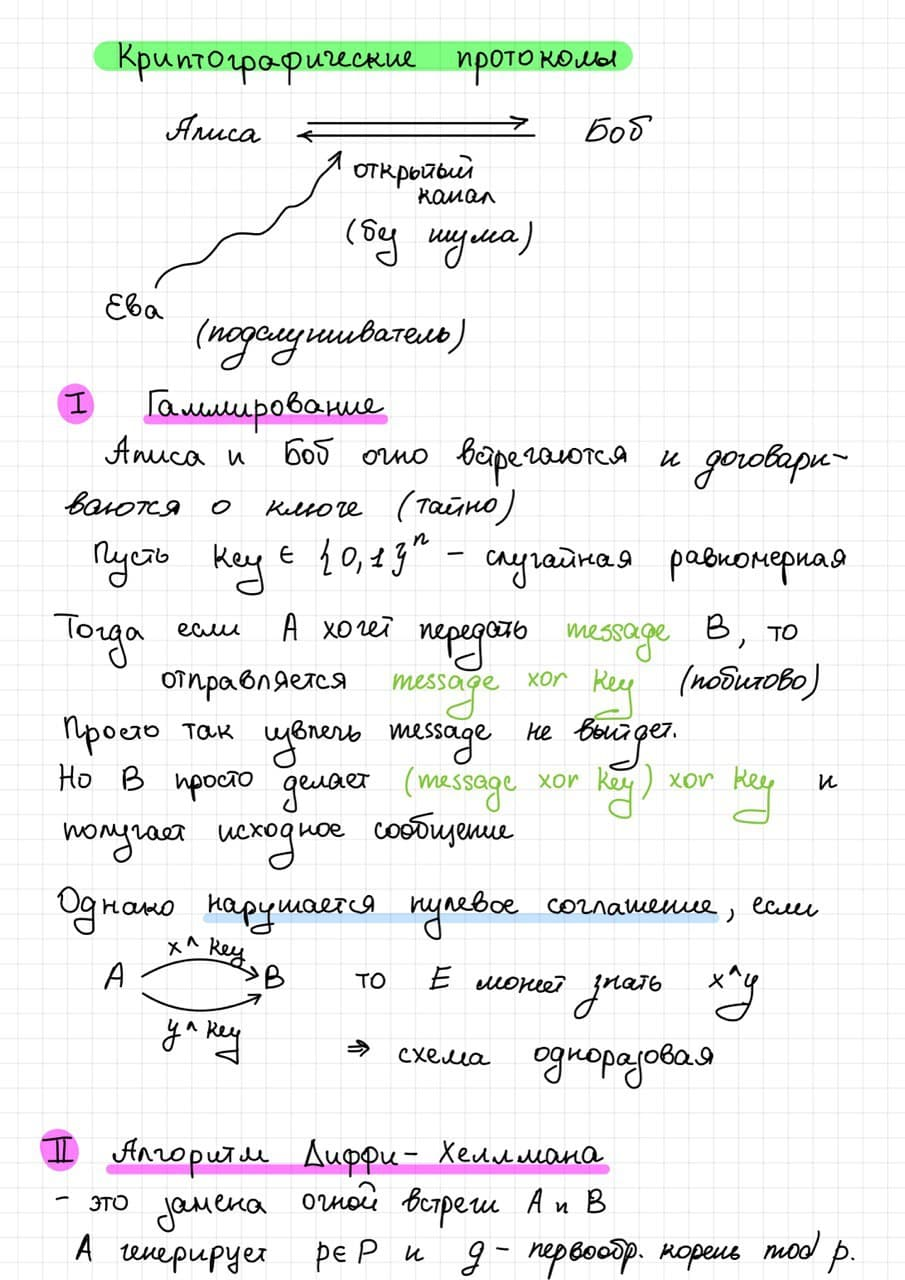
\includegraphics[width=1\linewidth]{images/Crypto1.jpg}
\newpage 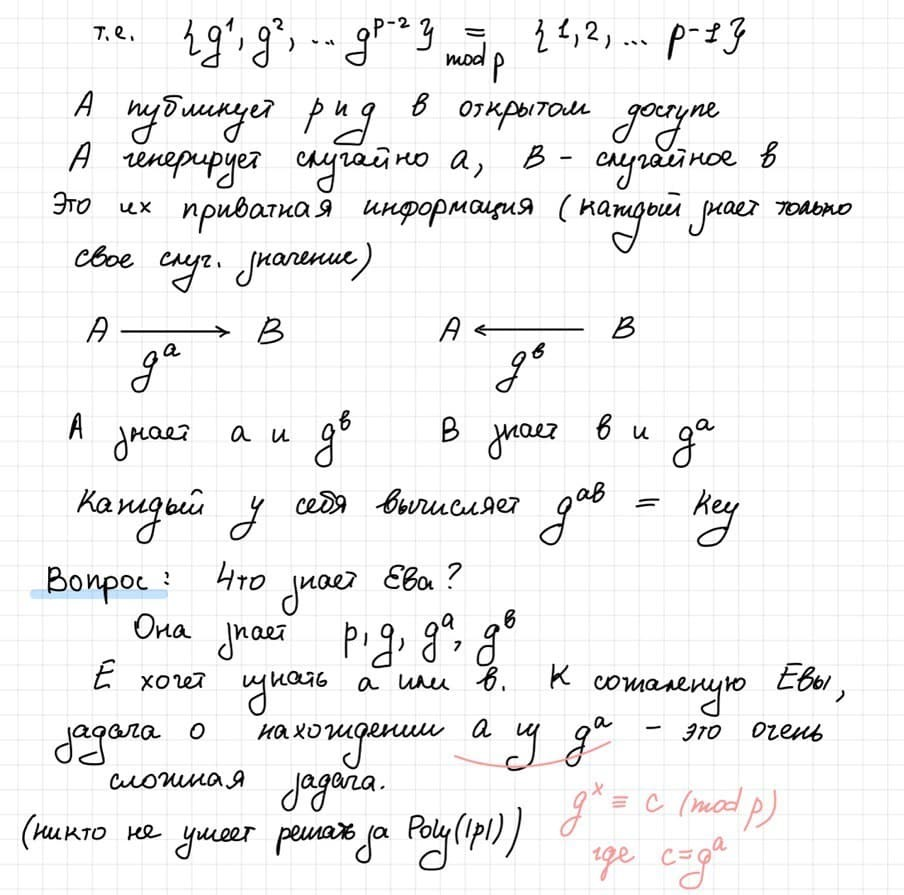
\includegraphics[width=1\linewidth]{Crypto2.jpg}

\section{Криптографический протокол RSA одностороннего общения. Неформальное доказательство надёжности протокола.}

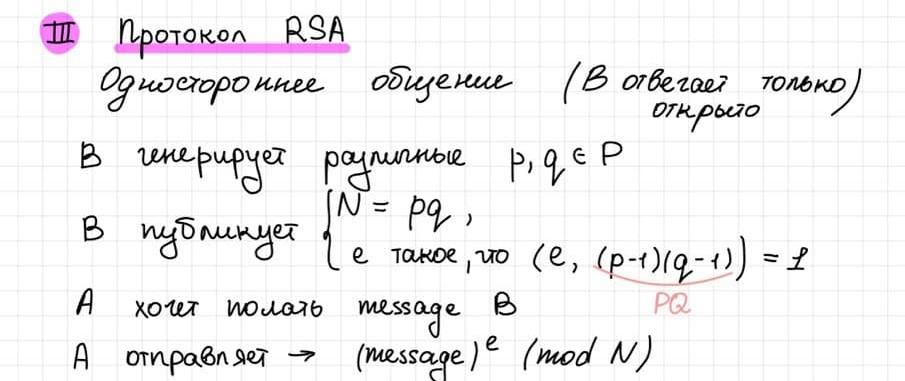
\includegraphics[width=1\linewidth]{images/Crypto3.jpg}
\newline 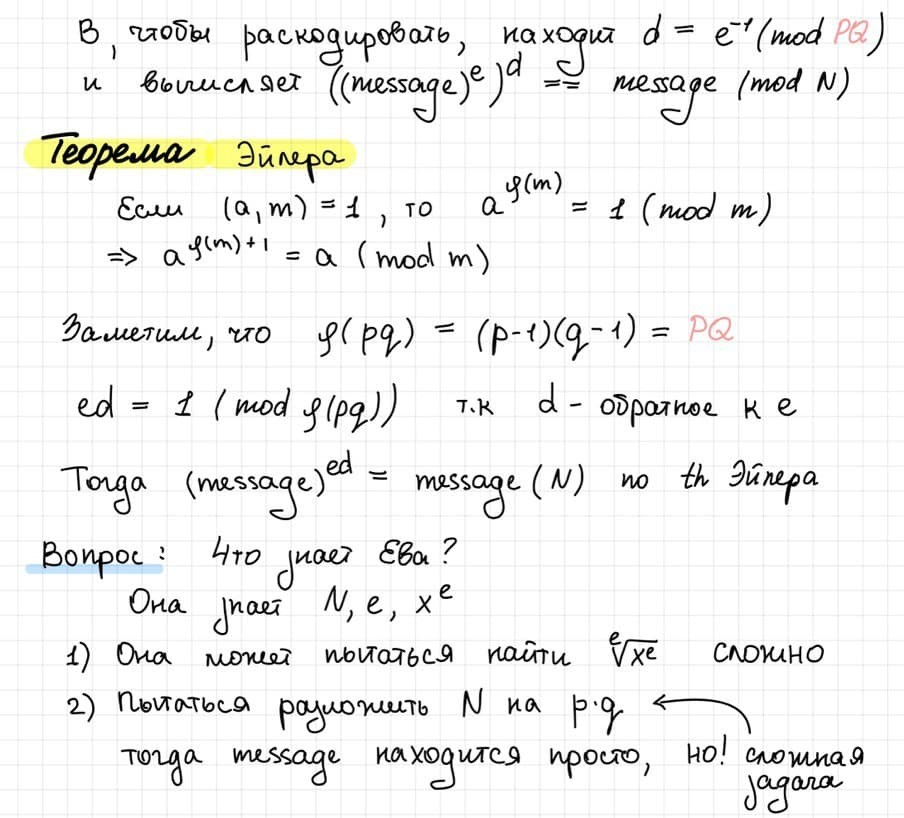
\includegraphics[width=1\linewidth]{Crypto4.jpg}

\section{Алгоритм Штрассена: постановка задачи, идея решения, асимптотика.}

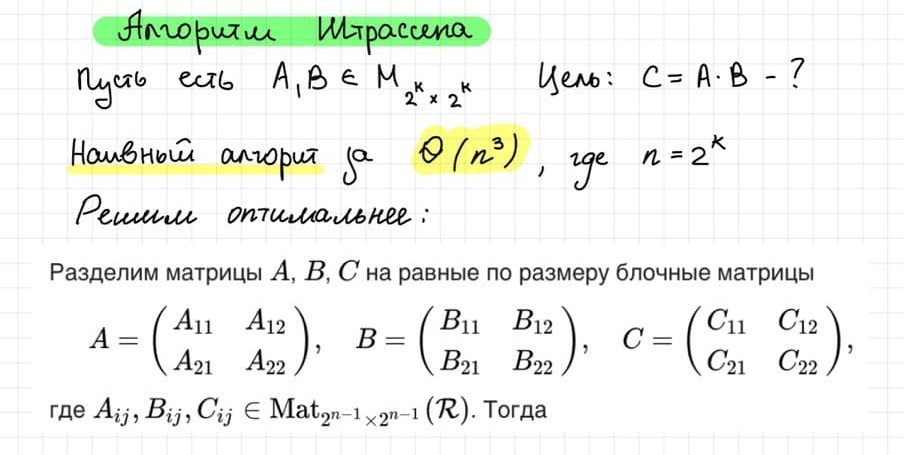
\includegraphics[width=1\linewidth]{images/Shtrassen1.jpg}
Продолжение на новой странице
\newpage 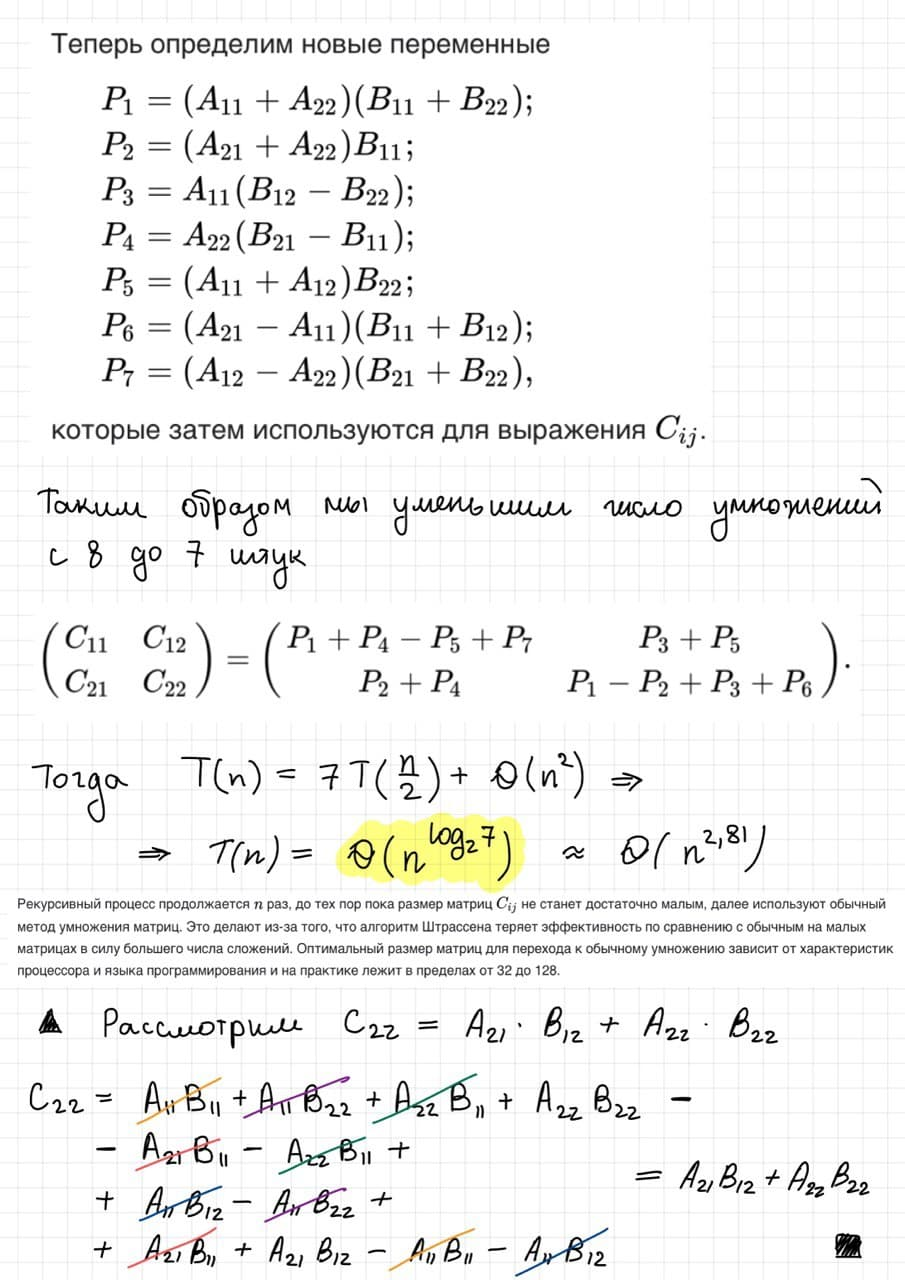
\includegraphics[width=1\linewidth]{images/Shtrassen2.jpg}

\section{Перемножение двух многочленов за O(n log n) с использованием быстрого преобразования Фурье как чёрного ящика.}

Пусть есть многочлен $P (x) = a_0 + a_1 x + \dots + a_{n - 1} x^{n - 1}$. Тогда $P$ однозначно восстанавливается по своим значениям в произвольных $n$ попарно различных точках. Это сводится к системе линейных уравнений:

\begin{center}
    $\left( \begin{matrix} x_1^0 & x_1^1 & \dots & x_1^{n - 1} \\ x_2^0 & x_2^1 & \dots & x_2^{n - 1} \\ \vdots & \vdots & \ddots & \vdots \\ x_n^0 & x_n^1 & \dots & x_n^{n-1} \end{matrix} \right) \left( \begin{matrix} a_0 \\ \vdots \\ \vdots \\ a_{n-1} \end{matrix} \right) = \left( \begin{matrix} y_1 \\ \vdots \\ \vdots \\ y_n \end{matrix} \right)$
\end{center}

Наша цель: перемножить $P$ и $Q$ и получить $R = P \cdot Q$. Будем делать это следующим образом:
\begin{itemize}
    \item Найдём $P ({x_1})$, $\dots$, $P({x_n})$. $Q ({x_1}$), $\dots$, $Q ({x_n})$ в некоторых точках $x_1$, $\dots$, $x_n$;
    \item $R ({x_i}) = P ({x_i}) \cdot Q ({x_i})$
    \item Восстановим $R$ по его значениям в $x_1$, $\dots$, $x_n$.
\end{itemize}

Чтобы все это работало, нужно чтобы:  $n \geqslant deg \ P + deg \ Q + 1$. Так как при $n > deg \ P + deg \ Q$ многочлен будет однозначно восстанавливаться по n точкам.
\\
\\
Осталось понять, в каких именно точках будем считать значения нашего многочлена. Удобно брать за $x_1$, $\dots$, $x_n$ — комплексные корни из $1$ степени $n$.
\\
\\
Нам нужно выбрать какое-то число, чтобы все его степени давали соответственно $x_1$, $\dots$, $x_n$. Тогда введём $\omega = e^{i \cdot \frac{2 \pi}{n}}$, $\omega^n = 1$. Получиим:
\begin{itemize}
    \item $x_1 = 1$
    \item $x_2 = e^{\frac{2 \pi i}{n}}$
    \item $\dots$
    \item $x_n = e^{\frac{2 \pi i(n-1)}{n}}$
\end{itemize}

Оценим асимптотику:
 \begin{itemize}
     \item  Первый шаг за счет быстрого преобразования Фурье будет делаться за O(n log n)
      \item Второй шаг - просто умножение за линию
      \item  Третий шаг - обратное преобразование Фурье. Так же O(n log n)
 \end{itemize}
\newpage{}

\section{Быстрое преобразование Фурье: рекурсивный алгоритм.}Как, собственно, будем делать Фурье.
\\ \\
Пусть нам дан многочлен $P (x) = a_0 + a_1 x + \dots + a_{n - 1} x^{n - 1}$
\\
\\
Вычислим $P ({\omega^0})$, $\dots$, $P (\omega^{n - 1})$. Для этого рассмотрим следующие многочлены:

\begin{itemize}
    \item  $P_0 (x) = a_0 + a_2 x + a_4 x^2 + a_6 x^3 + \dots$
    \item $P_1 (x) = a_1 + a_3 x + a_5 x^2 + a_7 x^3 + \dots$
\end{itemize}
Заметим, что $P (x) = P_0 (x^2) + x \cdot P_1 (x^2)$ (считаем, что n -  четно)
\\
\\
Тогда получается, что для того чтобы найти значение многочлена P во всех степенях $\omega$, достаточно найти значение $P_0$ и $P_1$ во всех четных степенях $\omega$
\\
\\
Если n - четно, то четных степеней $\omega$ ровно половина. Тогда достаточно найти значения $P_0$ и $P_1$ в точках $\omega^0, \ \omega^2, \ \omega^4, \ \dots, \ \omega^{n - 2}$.
\\
\\
Отсюда получим асимптотику: Найдём асимптотику: $T(n) = 2 T (\frac{n}{2}) + \Theta (n) \Longrightarrow T (n) = \Theta (n \log n)$.
\\ \\
\newpage{}

\section{Быстрое преобразование Фурье: обратное преобразование.}
Заметим, что вектор значений многочлена в точках ${\omega^0}$, $\dots$ $(\omega^{n - 1})$ может быть представлен в виде:

\begin{center}
    $\left( \begin{matrix} P(\omega^0) \\P(\omega^1) \\ \vdots \\ P(\omega^{n-1}) \end{matrix}\right)  = \left( \begin{matrix} \omega^{0 \cdot 0} & \omega^{0 \cdot 1} & \dots & \omega^{0 \cdot (n - 1)} \\ \omega^{1 \cdot 0} & \omega^{1 \cdot 1} & \dots & \omega^{1 \cdot (n - 1)} \\ \vdots & \vdots & \ddots & \vdots \\ \omega^{(n - 1) \cdot 0} & \omega^{(n - 1) \cdot 1} & \dots & \omega^{(n - 1) \cdot (n - 1)}   \end{matrix} \right)\left( \begin{matrix} a_0 \\ a_1 \\ \vdots \\ a_{n-1} \end{matrix}\right)$
\end{center}

Что мы сделали? По сути, мы умножили столбец коэффициентов на матрицу размера $n\times n$
\\
\\
Теперь мы хотим по столбцу значений восстановить столбец коэффициентов. Для этого нам достаточно умножить его на обратную матрицу. То есть: 
\begin{center}
 $\left( \begin{matrix} a_0 \\ a_1 \\ \vdots \\ a_{n-1} \end{matrix}\right)  = \left( \begin{matrix} \omega^{0 \cdot 0} & \omega^{0 \cdot 1} & \dots & \omega^{0 \cdot (n - 1)} \\ \omega^{1 \cdot 0} & \omega^{1 \cdot 1} & \dots & \omega^{1 \cdot (n - 1)} \\ \vdots & \vdots & \ddots & \vdots \\ \omega^{(n - 1) \cdot 0} & \omega^{(n - 1) \cdot 1} & \dots & \omega^{(n - 1) \cdot (n - 1)}   \end{matrix} \right)^{-1}\left( \begin{matrix} P(\omega^0) \\P(\omega^1) \\ \vdots \\ P(\omega^{n-1}) \end{matrix}\right) = \left( \begin{matrix} \omega^{0 \cdot 0} & \omega^{0 \cdot 1} & \dots & \omega^{0 \cdot (n - 1)} \\ \omega^{1 \cdot 0} & \omega^{1 \cdot 1} & \dots & \omega^{1 \cdot (n - 1)} \\ \vdots & \vdots & \ddots & \vdots \\ \omega^{(n - 1) \cdot 0} & \omega^{(n - 1) \cdot 1} & \dots & \omega^{(n - 1) \cdot (n - 1)}   \end{matrix} \right)^{-1}\left( \begin{matrix} c_0 \\c_1 \\ \vdots \\ c_{n-1} \end{matrix}\right)$
 \end{center}
 
 Сейчас  $(i,j)$ элемент нашей матрицы W - это $W_{ij} = \omega^{ij}$. Рассмотрим теперь матрицу V, которая определяется как $V_{ij} = (\omega^{-1})^{ij}$
 \\
 \\
 \textbf{Утверждение}
 \\
$W*V = n\cdot E_n$ \\
$\blacktriangle$
Рассмотрим i строку и j столбец матриц W и V соответственно.  Запишем их произведение \\ $\sum \limits_{k = 0}^{n - 1}w^{ik}*(w^{-1})^{kj} = \sum \limits_{k = 0}^{n - 1}w^{ik-kj} = \sum \limits_{k = 0}^{n - 1}w^{k(i-j)} = \frac{w^{n(i-j)} - 1}{w^{i-j} - 1}$
\\
Равно 0, если i!=j. В силу того, что $w^{n(i-j)} = 1$
\\
Если i = j, то последнее равенство не определено, и из предпоследнего делаем вывод, то сумма равна n. 
$\blacksquare$ \\ \\
Отсюда получаем, что $W^{-1} = \frac{1}{n}V$
\\
\\
Ну и все, почти победа. Выполним первый шаг, но с $\omega^{-1}$, после поделим каждый коэффициент на n. Получим, что нам надо.
\\
\\
\textit{Асимптотика: O(n log n), так как мы просто воспользовались первым шагом аглогитма (из прошлого билета) за O(n log n)}
\newpage{}

\section{Быстрое преобразование Фурье: избавление от рекурсии.}
В чем проблема? На практике рекурсия работает довольно медленно, поэтому от нее надо уходить
\\
Для начала маленький \textbf{пример}: \\
Посмотрим, как алгоритм будет работать на массиве длины 8: $[a_0, a_1, a_2, a_3, a_4, a_5, a_6, a_7]$
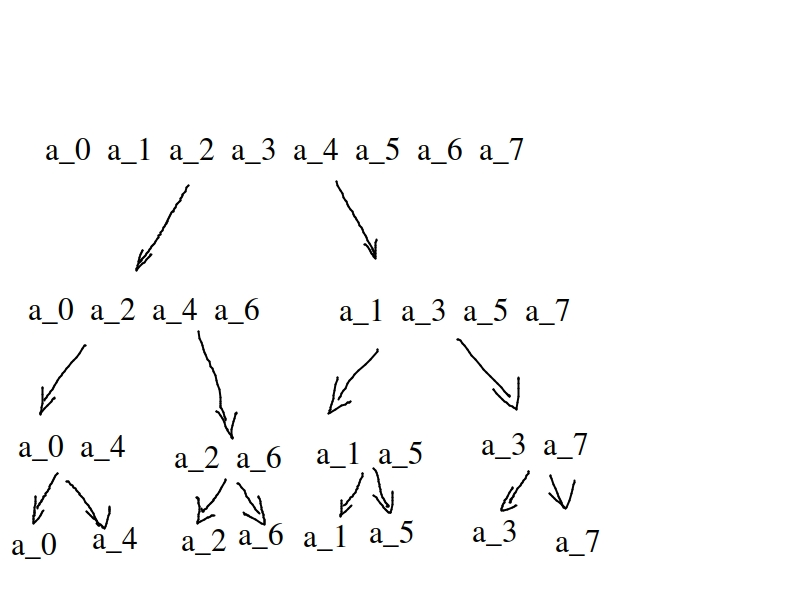
\includegraphics[width=10cm]{polina1.jpg}

На нижнем уровне у нас будут просто константы. То есть на нижнем уровне мы знаем значения многочленов в любой точке. Это просто свободный коэффициент
\\
\\
Теперь посмотрим на ячейку дерева, соответствующую $a_0 a_4$. Как вычислить значение для этого многочлена? 
\\
Многочлен на этом этапе выглядит как $a_0 + a_4 x$. Значения $\pm 1$. Получим значения $[a_0 + a_4, a_0 - a_4]$
\\
\\
Собственно, примерно это мы и хотим сделать. Как-то развернуть рекурсию снизу вверх так, чтобы уметь пересчитывать значения на более высоких уровнях, используя более низкие.
\\
\\
\\
Начнем это делать. \\
\textbf{Как заполнить нижкий ряд?} \\
\\
\textbf{Утверждение} \\
На i-м месте в массиве, соответствующем нижнему ряду, будет стоять коэффициент $a_{rev(i)}$, где rev(i) - это инверсия бит. \\  \\ Например, возьмем i = 1. Так как всего бит 3(в силу того, что $n = 2^3$), имеем rev(1) = rev(001) = 100 = 4
 \\
$\blacktriangle \\ $ В левое поддерево идут те элементы, у которых младший бит 0. Поэтому в терминах перевернутой записи имеем, что если у них был младший бит 0, то старший стал 0. Аналогично на втором этапе, влево идут те коэффициенты, чей второй младший бит 0, вправо - те, чей второй млдаший бит 1. Таким образом, мы полумаем сортировку по возрастанию перевернутых коэффициентов$ \\ \blacksquare $

Алгоритм пересчета rev за $O(n)$

\begin{lstlisting}
rev[0] = 0;
oldest = -1;
for (int mast = 1; mask < (1 << k); ++mask) {
  if (!(mask & (mask - 1))) {
    ++oldest;
  }
  rev[mask] = rev[mask ^ (1 << oldest)] | (1 << (k - oldest - 1));
}
\end{lstlisting}
Сложим эти значения в массив коэффициентов на нулевом уровне.
База у нас есть. 
\\
\textbf{Теперь как делать пересчет?}\\
Пусть мы знаем состояние массива на $j$-м снизу уровне. Разобьем массив на блоки размером $2^j$ и посчитаем блок $2^{j+1}$
\\
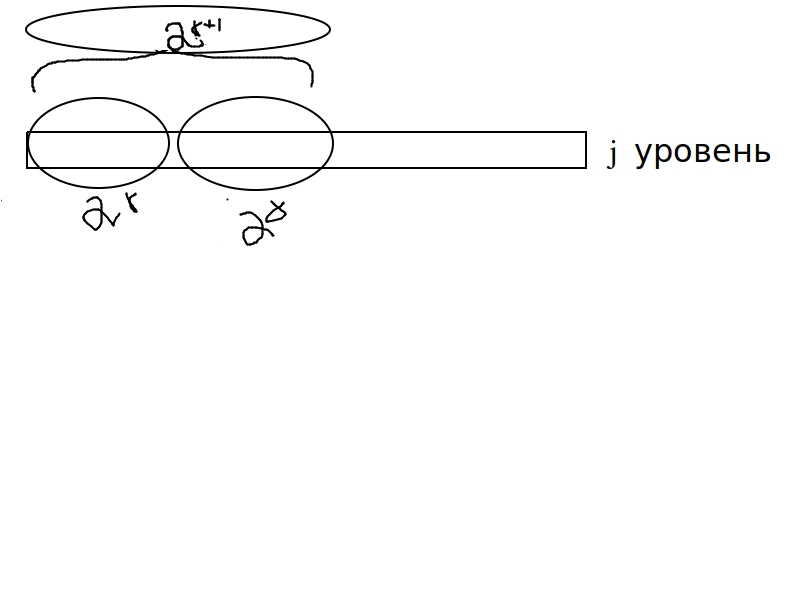
\includegraphics[width=10cm]{polina2.jpg}\\
 Рассмотрим многочлен $T (x) = a_i + a_{i + 1} x + \dots + a_{i + 2^{j^{i + 1}} - 1} \cdot x^{2^{j^{i + 1}} - 1}$. Его можно найти, зная его разбиение на $T_0$ и $T_1$: $T (x) = T_0 (x^2) + x \cdot T_1(x^2)$. Найдём $T (\omega^0)$, $\dots$, $T (\omega^{j - 1})$. Считаем $s < \frac{j}{2}$, тогда: 

\begin{center}
    $T (\omega^s) = T_0 (\omega^{2s}) + \omega^s \cdot T_1 (\omega^{2s})$
    
    $T (\omega^{\frac{j}{2} + s}) = T_0 (\omega^{2s + j}) + \omega^{\frac{j}{2} + s} \cdot T_1 (\omega^{2s + j}) = T_0(\omega^{2s}) - \omega^s \cdot T_1 (\omega^{2s})$.
\end{center}
\begin{lstlisting}
for (int len=2; len<=n; len<<=1) {
		double ang = 2*PI/len;
		base wlen (cos(ang), sin(ang));
		for (int i=0; i<n; i+=len) {
			base w (1);
			for (int j=0; j<len/2; ++j) {
				base u = a[i+j],  v = a[i+j+len/2] * w;
				a[i+j] = u + v;
				a[i+j+len/2] = u - v;
				w *= wlen;
			}
		}
	}
\end{lstlisting}
\newpage{}

\section{Примитив точки, вектора, прямой. Построение прямой по двум точкам.}

\subsubsection*{Точка и вектор}

В $R^2$ можно задать декартовую систему координат, обладающей осями абсцисс и ординат. Каждую точку можно задать двумя координатами $(a, b)$, обозначающие проекцию на каждую из осей. Каждой точке можно сопоставить радиус вектор из $(0, 0)$ в $(a, b)$. Для точки заведём структуру point:

\begin{lstlisting}
struct point {
  int x, y;
};
\end{lstlisting}


Пусть у нас есть вектор $\vec{v}$ из точки $p$ в точку $q$. Его можно задать как $(q.x - p.x, q.y - p.y)$. Для структуры point можно написать оператор «минус»:

\begin{lstlisting}
point operator - (const point& other) const {
  return {x - other.x, y - other.y}
}
\end{lstlisting}

Можно также реализовать оператор «плюс», соответствующее сложению векторов, а также оператор «звёздочка» умножения на скаляр.

\subsubsection*{Прямая}

Далее нам пригодится примитив «прямая», и мы хотим, чтобы она однозначно задавалась. Удобно её представлять в виде $y = kx + b$, но есть проблема: вертикальные прямые так не задаются. Можно было бы повернуть на случайный угол $\alpha$. Но с целыми числами возможна проблема. Поэтому будем представлять прямую в виде $ax + by + c = 0$:

\begin{lstlisting}
struct line {
  int a, b, c;
};
\end{lstlisting}

Но есть проблема: прямая может задаваться неоднозначно. Чтобы убедиться в этом, достаточно умножить обе части на $\lambda$. 

Удобно строить прямую по двум точкам:

\begin{lstlisting}
line (const point& p, const point& q) {
  if (p == q) {
    exception;
  }
  a = p.y - q.y;
  b = q.x - p.x;
  c = p.x * q.y - p.y * q.x;
}
\end{lstlisting}

Действительно, если есть две точки $p(x_1, y_1)$, $q(x_2, y_2)$, то $a = y_1 - y_2$, $b = x_2 - x_1$, $c = x_1 y_2 - x_2 y_1$. Доказывается подстановкой точек $p$ и $q$ в уравнение $ax + by + c = 0$;

С прямой $ax + by + c = 0$ связаны два вектора: вектор нормали $\vec{n} (a, b)$ и направляющий вектор $\vec{l} (b, -a)$, можно взять как $(-b, a)$. 

\newpage{}

\section{Расстояние от точки до прямой, проекция. Пересечение двух прямых.}
$H = (V, E)$ - $n$-однородный гиперграф. (при $n = 2$ это обычный граф)
Пусть $k$ - максимальная степень вершины.

\Def Раскраска множества вершин $V$ гиперграфа $H = (V, E)$ называется правильной, если в этой раскраске все ребра из $E(H)$ не являются одноцветными. Хроматическим числом гиперграфа $H$ называется минимальное число цветов, требуемое для правильной раскраски вершин этого гиперграфа. 
\\
\\
$X(H)$ - хроматическое число гиперграфа \\
При $n = 2 \Rightarrow X(H) \leq k + 1$ (Тривиальная оценка для обычных графов) \\
При $n \geq 3 \Rightarrow X(H) \leq f(kn)$, где $f$ - какая-то функция.

\Th $e \cdot r^{1-n}(n(k-1)+1)  \leq 1 \Rightarrow X(H) \leq r$ (ничего лучшего для $n \geq 3$ сейчас не знают).

\Proof

Красим гиперграф в $r$ цветов

Красим каждую вершину в каждый конкретный цвет с вероятностью $\frac{1}{r}$.

Пусть $e_1, ..., e_{|E|}$ - рёбра гиперграфа

$A_1, ..., A_{|E|}$, где $A_i$ - событие: $e_i$ - одноцветное.

Если докажем, что $P(\bigcap_{i=1}^{|E|} \overline{A_i}) > 0$, получим $X(H) \leq r$, потому что докажем возможность покраски графа в $r$ цветов, не получив одноцветные рёбра. Докажем это:

$p = P(A_i) = r^{1-n}$

$d$ - число зависимостей. $d \leq n \cdot (k - 1)$ (Это суммарная степень всех вершин, помимо выбранного ребра(события))

По условию теоремы $e \cdot r^{1-n}(n(k-1)+1) \leq 1$, следовательно выполняется неравенство $e p (d + 1) \leq 1$. Можем воспользоваться ЛЛЛ и получить $P(\bigcap_{i=1}^{|E|} \overline{A_i}) > 0 \Rightarrow X(H) \leq r  \ \blacksquare$

$(e(n(k-1)+1))^{\frac{1}{n-1}} \leq 1 \Rightarrow X(H) \leq r$ 

$(e(n(k-1)+1))^{\frac{1}{n-1}} \leq 1 \Rightarrow r \geq \left\lceil (e(n(k-1)+1))^{\frac{1}{n-1}} \right\rceil$

И если взять в качестве $r$ значение $\left\lceil (e(n(k-1)+1))^{\frac{1}{n-1}} \right\rceil$, то оно будет удовлетворять условию $r \geq \left\lceil (e(n(k-1)+1))^{\frac{1}{n-1}} \right\rceil$ (переформулированное начальное условие), следовательно, применима теорема. Получим оценку $X(H) \leq \left\lceil (e(n(k-1)+1))^{\frac{1}{n-1}} \right\rceil$.

Если подставить n = 2 (то есть граф обычный), то получим $X(H) \leq \left\lceil e(2(k-1)+1) \right\rceil$

Эта оценка хуже, чем обычная: $X(H) \leq k + 1$, но сопостовимая.
\newpage{}

\section{Примитив окружности. Пересечение прямой и окружности. Пересечение двух окружностей.}

\subsubsection*{Примитив окружности}

Окружность можно хранить как пару: точка $p$, отвечающая за центр окружности, и её радиус $r$.

\subsubsection*{Пересечение окружности и прямой}

Пересечение окружности и прямой $l$ есть тогда и только тогда, когда расстояние между центром окружности и прямой $l$ не превосходит $r$. Можно полагать, что мы ищем решение системы уравнений:

\begin{center}
    $\begin{cases}
    ax + by + c = 0; \\
    (x - x_0)^2 + (y - y_0)^2 = r^2
    \end{cases}$
\end{center}

Найдём $q$ - проекцию точки $p$ на прямую. (для этого можно опустить перпендикуляр из центра окружности на прямую.) Далее отступим от проекции $q$ на некоторое расстояние по обе стороны. Для этого найдём направляющий вектор прямой $l$, нормируем его. Найдём $k = \sqrt{r^2 - {dist}^2 (p, q)}$, где $dist (p, q) = \sqrt{(p.x - q.x)^2 + (p.y - q.y)^2}$. Находим $q + k \vec{v}$, $q - k \vec{v}$, где $\vec{v}$ — направляющий вектор $l$ единичной длины. Это и есть искомые точки.

\subsubsection*{Пересечение двух окружностей}

Пусть заданы две окружности: одна с центром в точке $(x_1, y_1)$ и радиусом $r_1$; другая с центром в точке $(x_2, y_2)$ и радиусом $r_2$. Можно полагать, что мы ищем решение системы уравнений:

\begin{center}
    $\begin{cases}
        (x - x_1)^2 + (y - y_1)^2 = r_1^2; \\
        (x - x_2)^2 + (y - y_2)^2  = r_2^2.
    \end{cases}$
\end{center}

Вычтем второе уравнение из первого.

\begin{center}
    $\begin{cases}
        (2x_2-2x_1)x + (2y_2-2y_1)y + (x^2_1 - x^2_2 + y^2_1 - y^2_2 + r^2_2 - r_1^2) = 0; \\
        (x - x_2)^2 + (y - y_2)^2  = r_2^2.
    \end{cases}$
\end{center}

Свели задачу к поиску точки пересечения окружности и прямой.

Здесь не обойтись без чисел с плавающей точкой.

\newpage{}

\section{Ушная триангуляция многоугольника: лемма о двух ушах.}
Есть некоторый многоугольник — замкнутая несамопересекающаяся ломаная. Нужно найти его триангуляцию — разбиение многоугольника на треугольники с помощью диагоналей такое, что все эти треугольники лежат в многоугольники. Диагонали здесь являются отрезками между несоседними вершинами, полностью лежащие во внутренности многоугольника.

Вершина $v_i$ называется ухом, если диагональ $v_{i-1}v_{i+1}$ лежит строго во внутренней области многоугольника P

Лемма о двух ушах: У любого простого n-вершинного многоугольника P всегда существует два не пересекающихся между собой уха.

Доказательство будем вести по индукции. Базовый случай: $n=4$. Предположим для всех многоугольников, количество вершин в которых не больше $n$, теорема верна. Рассмотрим многоугольник P, в котором $n+1$ вершина. Далее возможны два случая:
\begin{enumerate}
    \item Случай, когда $v_i$ является ухом в P. \\
    Произвольная выпуклая вершина $v_i$ многоугольника P является ухом. Отрезав это ухо, мы уменьшим число вершин P на одну. В результате, получим n-вершинный многоугольник P'. По предположению индукции у него существует два непересекающихся уха. Учитывая, что уши P' являются ушами и P, несложно заметить, что для P теорема верна.
    \item Произвольная выпуклая вершина $v_i$ многоугольника P не является ухом. \\
    В таком случае в треугольнике $\Delta v_{i-1}v_iv_{i+1}$ лежат вершины, принадлежащие P. Из этих вершин выберем вершину q, которая будет ближе всего к $v_i$. Проведём отрезок Q, который разделит P на два многоугольника: $P_1$ и $P_2$. В каждом из них будет не более n вершин, следовательно у каждого будет по два непересекающихся уха. Даже если предположить, что ухо из $P_1$ и ухо из $P_2$ будут пересекаться по стороне $v_{iq}$, в P всё равно будет не менее двух непересекающихся ушей.
\end{enumerate}

\section{Алгоритм триангуляции многоугольника за $O(n^2)$, где n — число вершин.}
Рассмотрим алгоритм построения триагнуляции.

Поддерживаем вершины многоугольника в двусвязном списке. Далее напишем процедуру $FindEar$, которая проводит отрезок между $v_{i + 1}$ и $v_{i - 1}$ и смотрит, попали ли ещё точки внутри. Если нет, то это ухо, иначе найдём точку внутри треугольника, и проведём диагональ. Точек найдётся не более, чем $\frac{n}{2} + 1$. Далее запустимся рекурсивно. Найдём асимптотику, пользуясь мастер-теоремой: $T (n) = \Theta(n) + T (\frac{n}{2}) \Longrightarrow T (n) = \Theta (n)$.

Алгоритм весь будет работать за $\Theta (n^2)$. Существует алгоритм за $O (n \log n)$, который, скорее всего, рассмотрен не будет.

Поиск в Боре:
При решении этой задачи, обход бора совершается из его корня по рёбрам, отмеченным символами строки $S$, пока возможно. Если с последним символом $S$ мы приходим в терминальную вершину, то $S$ — слово из словаря. Если в какой-то момент ребра, отмеченного нужным символом, не находится, то строки $S$ в словаре нет. Ясно, что это занимает $O(|S|)$ времени. Таким образом, бор — это эффективный способ хранить словарь и искать в нем слова.

\section{Выпуклая оболочка конечного множества точек: определение и доказательство того, что выпуклая оболочка — многоугольник.}

\Def Пусть $\vec{u} = (x_1, y_1)$, $\vec{v} = (x_2, y_2)$. «Векторным»  произведением $\vec{u} \times \vec{v} = [\vec{u}, \vec{v}] = cross (\vec{u}, \vec{v})$ называется величина $x_1 y_2 - x_2 y_1 = \bigg| \begin{matrix} 
x_1 & x_2 \\ 
y_1 & y_2 
\end{matrix} \bigg|$.

Свойства «векторного произведения»:

\begin{enumerate}
    \item Его величина численно равна ориентированной площади параллелограмма, натянутого на векторы $\vec{u}$ и $\vec{v}$;
    \item $\vec{u} \times \vec{v} = |u| \cdot |v| \cdot \sin \alpha$;
    \item Знак векторного произведения говорит нам о направлении кратчайшего поворота между двумя векторами: если знак положительный, то против часовой стрелки, если знак отрицательный, то по часовой стрелке, если значение равно нулю, то векторы либо сонаправлены, либо направлены противонаправлены.
\end{enumerate}

\Def Пусть $S$ — множество точек в $\mathbb{R}^2$, $|S| = n$. Тогда выпуклой оболочкой $S$ называется минимальное по включению пересечение выпуклых надмножеств $S$: $conv (S) = \bigcap \limits_{F \supset S} F$, где $F$ — выпуклое множество (поскольку является пересечением выпуклых множеств).

\begin{minipage}[r]{0.15\linewidth} 
%\begin{flushright}
    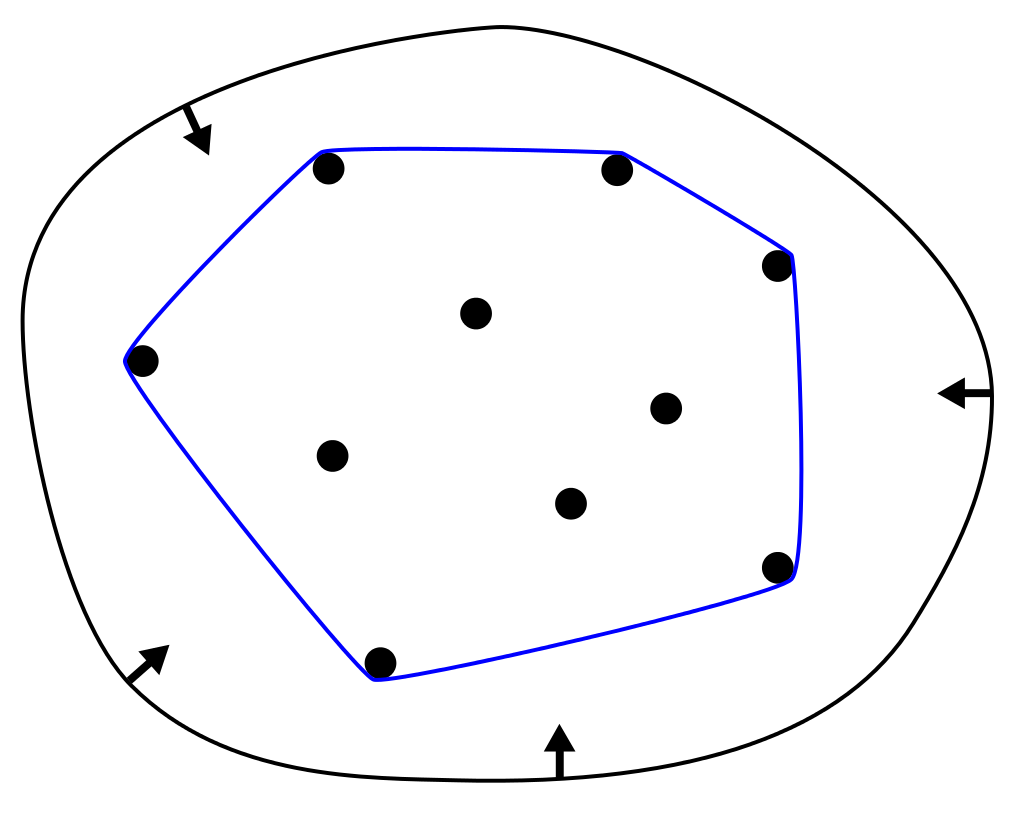
\includegraphics[width=2\linewidth]{images/44_1.png}
%\end{flushright} 
\end{minipage} \\

\Def Напомним определение выпуклости -- если две точки лежат в множестве, то и отрезок, их соединяющий тоже лежит в множестве.

\Note $conv (S)$ — минимальное по включению выпуклое множество, содержащее $S$.

\Note $conv (S)$ — выпуклый многоугольник (в вырожденных случаях — отрезок или точка) с вершинами в некоторых точках $S$.\\

\textit{Почему выпуклая оболочка -- многоугольник с вершинами в точках множества (выпуклость уже известна):}\\
\Proof Докажем по индукции, почему это многоугольник с вершинами в точках множества.
\begin{enumerate}
    \item Для $n = 1$ утверждение очевидно (это точка), для $n = 2$ -- тоже (отрезок).
    \item Пусть верно для $n$, докажем для $n + 1$. Для этого из нашего множества на $n + 1$ точке временно уберем одну из них (пусть это точка $A$). Для оставшихся точек утверждение верно, построим для них выпуклую оболочку $G$. Далее соединим точку $A$ со всеми точками из $G$.
    
    Заметим, что полученная фигура $G_2$ -- выпуклая. Докажем это. Возьмем две точки $X$ и $Y$ из $G_2$. Они лежат на отрезках $AB$ и $AC$ соответственно, где точки $B$ и $C$ -- из множества $G$.
    
    Заметим, что т.к. отрезок $BC$ целиком лежит в $G$, то он лежит и в $G_2$. А тогда и весь треугольник $ABC$ лежит в $G_2$. В частности, и отрезок $XY$.
    
    Из построения видно, почему выпуклая оболочка лежит в $G_2$. Далее поймем, что $G_2$ лежит в выпуклой оболочке (т.к. $G$ и все проведенные отрезки обязаны лежать в выпуклой оболочке). Значит, они совпадают. 
    
    Также из построения видно, что $G_2$ -- многоугольник. (Если точка $A$ лежала внутри или на границе $G$, то это очевидно, а если нет, то заметим, что $G_2$ является объединением треугольников, построенных на соседних вершинах $G$ и вершине $A$).
\end{enumerate}
\EndProof
\newpage{}

\section{Построение выпуклой оболочки заворачиванием подарка за O(nh).}

Этот алгоритм работает за $O (nh)$, где $h$ — число вершин в выпуклой оболочке. Рассмотрим точку из $S$ с минимальной ординатой. Если таких несколько, то выберем из них точку с минимальной абсциссой. Заметим, что эта точка точно должна лежать в выпуклой оболочке.

Если мы возьмем точку, которая образует минимальный полярный угол с последней найденной стороной выпуклой оболочки (считая от стороны), эта точка тоже точно будет лежать в выпуклой оболочке.
Каждый раз в порядке угла будем добавлять точки в выпуклую оболочку, и поддерживать
выпуклую оболочку для данных точек. Причем, при равестве углов нас будет интересовать максимально удаленная от последней вершины точка.

\begin{minipage}[r]{0.2\linewidth} 
%\begin{flushright}
    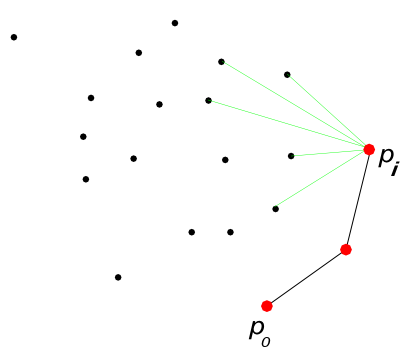
\includegraphics[width=2\linewidth]{images/45_1.png}
%\end{flushright} 
\end{minipage} \\

Заметим, что когда мы сравниваем по углу, нам достаточно знать кто правее, а точный угол знать не надо. Можно использовать для этого векторное произведение.

\textit{Корректность:} Точка $p_0$, очевидно, принадлежит оболочке. На каждом последующем шаге алгоритма мы получаем прямую $p_{i-1}p_i$, по построению которой все точки множества лежат слева от нее.\\
Значит, выпуклая оболочка состоит из $p_i$-ых и только из них.\\

\textit{Асимптотика:} Добавление каждой точки в ответ занимает $O(n)$ времени, всего точек будет $h$, поэтому итоговая сложность $O(nh)$. В худшем случае, когда оболочка состоит из всех точек сложность $O(n^2)$.

\newpage{}

\section{Построение выпуклой оболочки сортировкой точек по координатам за $O(n\log n)$.}

Алгоритм:

\begin{itemize}
    \item Отсортируем $S$ по парам $(x, y)$ сначала по возрастанию $x$, затем по возрастанию. $y$
    \item Строим нижнюю и верхнюю части выпуклой оболочки. Определим крайние левую и правую точку текущей оболочки. В отдельных векторах будем хранить нижнюю и верхнюю часть.\\
    
    При рассмотрении новой вершины $N$ проводим касательные к оболочке через неё. Пусть это $NA$ и $NB$ (Касательные будут проходить через какие-то вершины выпуклой оболочки $A$ и $B$). Заметим, что эта вершина обязана лежать в новой выпуклой оболочке (т.к. она самая правая). А все вершины, которые попали в угол $ANB$ и раньше лежали в оболочке, теперь должны быть из нее удалены, потому что больше не будут в ней участвовать (они покрываются новой фигурой).
    
    Чтобы было понятнее, рассмотрим картинку:
    
    \begin{minipage}[r]{0.2\linewidth} 
    %\begin{flushright}
        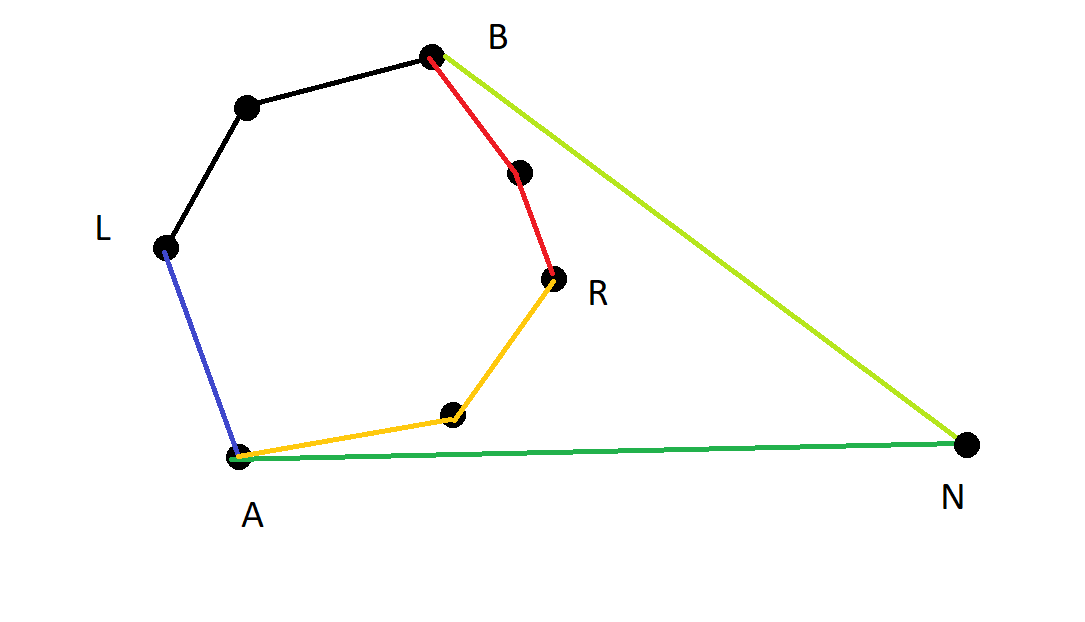
\includegraphics[width=2\linewidth]{images/46_1.png}
    %\end{flushright} 
    \end{minipage} \\
    
    На этой картинке черным показан тот кусок верхней части оболочки, который останется, красный же кусок будет удален. Вместо него добавится светло-зеленый (наша касательная).
    Для нижней части аналогично: синим помечен кусок, который останется, желтым, который будет удален, а темно-зеленым тот, который добавится.\\
    
    Почему именно мы хотим удалять вершины внутри угла? Идея такая же, как в алгоритме заворачивания подарка. 
    
    Рассмотрим нижнюю половину. Для нее векторы сторон отсортированы по углу против часовой стрелки. Мы хотим, чтобы вновь добавленная вершина не портила нам выпуклость, то есть вектор в нее из последней точки должен идти за предыдущим в порядке поворота именно против часовой стрелки (положительное векторное произведение). Поэтому нам достаточно удалять с конца вершины из нижней половины до тех пор, пока векторное произведение отрицательно.\\
    
    Аналогично для верхней половины (но только знаки нужно поменять на противоположные).
    
    \item Добавим вершину в каждую из половин

\end{itemize}
 
В конце нужно будет лишь слить две части оболочки (не забыв, что самую левую и самую правую точку мы посчитали в двух экземплярах -- в каждой из частей, а потому у них нужно удалить по одному экземпляру).\\

\textit{Асимптотика:}

Асимптотика $O(n\log n)$ достигается за счёт сортировки в самом начале. В оставшейся части алгоритма у нас асимптотика $O(n)$, поскольку каждую вершину мы добавляем и удаляем не более одного раза. А не добавляя и не удаляя, вершины мы расматриваем только в случае, если через них проходят наши касательные, а это 2 лишних действия на каждом шаге (которых $O(n)$).
\newpage{}

\section{Построение выпуклой оболочки сортировкой точек по полярному углу за O(n log n).}

\begin{enumerate}
    \item Находим точку $p_0$ нашего множества с самой маленькой $y$-координатой (если таких несколько, берем самую левую из них), добавляем в ответ.
    \item Сортируем все остальные точки по полярному углу относительно $p_0$.
    \item Добавляем в ответ $p_1$ - самую первую из отсортированных точек.
    \item Берем следующую по счету точку $t$. Пока $t$ и две последних точки в текущей оболочке $p_i$ и $p_{i-1}$ образуют неправый поворот (вектора $p_it$ и $p_{i-1}p_i$), удаляем из оболочки $p_i$.
    \item Добавляем в оболочку $t$.
    \item Делаем п.5, пока не закончатся точки.
\end{enumerate}

Иллюстрация:

Черные ребра уже лежат в выпуклой оболочке. При добавлении в нее вершины $p_{i + 3}$ мы вынуждены удалить вершины $p_{i + 1}$ и $p_{i + 1}$ из оболочки.\\

\begin{minipage}[r]{0.3\linewidth} 
%\begin{flushright}
    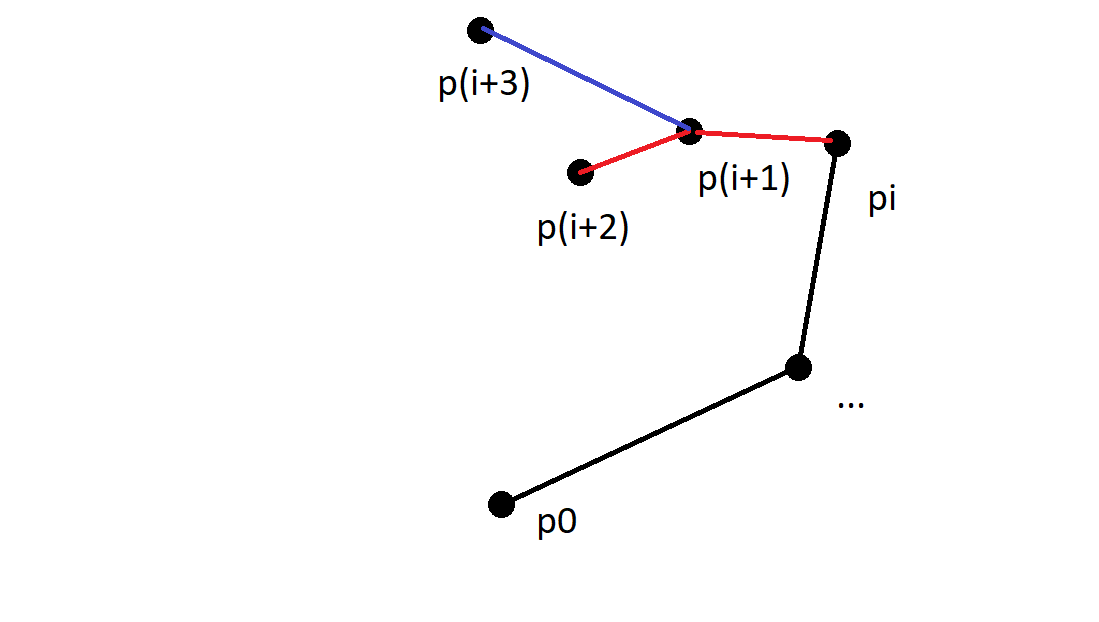
\includegraphics[width=2\linewidth]{images/47_1.png}
%\end{flushright} 
\end{minipage} \\

Теперь, как такое реализовывать

1. Перемещаем многоугольник в начало координат(из всех вершин вычитаем самую нижнюю,
левую точку).
2. Сортируем все точки по полярному углу.
Заметим, что нам достаточно знать кто правее, а точный угол знать не надо. Можно использовать для этого векторное произведение.
Если углы равны, то нужно сравнивать по длине, сначала рассматривать точки, которые ближе к начальной, а потом те, что дальше.

\begin{lstlisting}
1 bool cmp(Point A, Point B) {
2 if (cross_product(A, B) > 0) return 1;
3 else return A.len < B.len // заметим, что нам не нужно извлекать корень, для сравнения 4 
4 }
\end{lstlisting}

3. Теперь, для построения самой выпуклой оболочки, кладем все в стек.
При обработки новой точки, если при добавление точки выпуклость не портится, то все хорошо, если выпуклость портится с последними точками, то выкидываем последнюю точку и проверяем еще раз до тех пор, пока добавление не станет корректным (а оно точно станет).

4. Добавляем новую точку в стек.\\

\textit{Корректность:}

\Proof
Докажем, что на каждом шаге множество $p_i$-тых является выпуклой оболочкой всех уже рассмотренных точек. Доказательство проведем по индукции.

База. Для трех первых точек утверждение, очевидно, выполняется.

Переход. Пусть для $i-1$ точек оболочки совпадают. Докажем, что и для $i$ точек они совпадут.
Рассмотрим истинную оболочку $C_i$. Так как мы добавляли точки в нашу оболочку против часовой стрелки и так как $i$-тая точка лежит в $C_i$, то множество точек $C_{i-1}$, которые попадут внутрь $C_i$ состоит из нескольких подряд идущих последних добавленных в оболочку точек, и именно их мы удаляем на текущем шаге. Поэтому на $i$ шаге мы получим выпуклю оболочку для рассматриваемых на этом шаге точек. 

\EndProof

\textit{Асимптотика:}

Сортировка точек занимает $O(n\log n)$ времени. При обходе каждая точка добавляется в ответ не более одного раза, поэтому сложность этой части - $O(n)$. Суммарное время — $O(n \log n)$.
\newpage{}

\section{Максимум скалярного произведения с фиксированным вектором, нахождение за O(log n).}

Дано множество $S$ векторов (точек) мощности $n$. Поступает запрос вида <<найти точку (из данных) $(x, y)$ такую, что $(x, y) \cdot (a, b)$ максимально>>, где $a, b$ -- даны.

\Statement Скалярное произведение достигает своего максимального значения только на границе выпуклой оболочки множества точек $S$.

\Proof
Заметим, что на прямой, перпендикулярной вектору, скалярные произведения одинаковы. Поэтому для любой точки внутри выпуклой оболочки можно продлить перпендикуляр до точки пересечения с границей. Тогда значение для одного из концов отрезка, на который точка пересечения попадет, будет не меньше.

\EndProof

Разобьем нашу выпуклую оболочку на две части -- верхнюю и нижнюю. Для $b \geq 0$ будем искать ответ в верхней половине, иначе в нижней. 

\textit{Факт, который не доказывался на лекции:}

Скалярное произведение сначала увеличивается, потом (возможно) остается константным некоторое время (если есть отрезок, перпендикулярный вектору), а потом уменьшается.

Поэтому точку, когда скалярное произведение максимально, можно искать бинпоиском -- если скалярное произведение увеличивается в точке, двигаем левую границу, иначе -- правую.

\textit{Асимптотика:} $O(\log n)$ из-за бинпоиска.
\newpage{}

\section{Динамическая выпуклая оболочка: вставка точек за O(log n)}

Пусть дано множество точек $S$, изначально пустое, и набор точек ${p_i}^n_{i=1}$, которые последовательно добавляются в $S$. Требуется динамически поддерживать выпуклую оболочку $S$.

Идея: пытаемся использовать касательные, как в алгоритме поиска выпуклой оболочки через сортировку по координатам.\\

Снова разобьем выпуклую оболочку на две части -- верхнюю и нижнюю. Будем хранить каждую из них в своем $set$.

Вот нам приходит новая точка. Пусть она лежит снаружи выпуклой оболочки. Тогда проведем 2 касательные из этой точки к оболочке. Как ма ранее (в 46 билете) доказывали, нам необходимо удалить только точки, которые находятся между <<точками касания>>. 

Проблема: это может быть где-то вообще в середине.\\

Решение: Рассмотрим сначала верхнюю часть. Бинпоиском (методом $lower\_bound$) найдем, между какими точками по координате $x$ лежит вновь пришедшая точка (назовем ее N). Крайний случай -- когда она левее или правее всех.\\ 

Заметим, что верхнюю часть не нужно менять только, если точка $N$ лежит ниже, чем граница верхней части выпуклой оболочки, или на этой границе. Это, кстати, довольно просто проверить -- достаточно пересечь отрезок выпуклой оболочки (между концами которого попала точка) с вертикальной прямой с координатой нашей точки. И сравнить их ординаты.

Если же точка левее или правее всех, то менять в любом случае придется.\\

Заметим, что удаляются только последние несколько точек подряд с координатой $x$ меньше, чем у $N$, и первые несколько точек с координатой $x$ больше, чем у $N$. В случае, когда $N$ -- крайняя, удаляются точки только с одной стороны. \\

Аналогично поступим с нижней частью (только знаки в сравнениях будут в другую сторону).

\begin{minipage}[r]{0.3\linewidth} 
%\begin{flushright}
    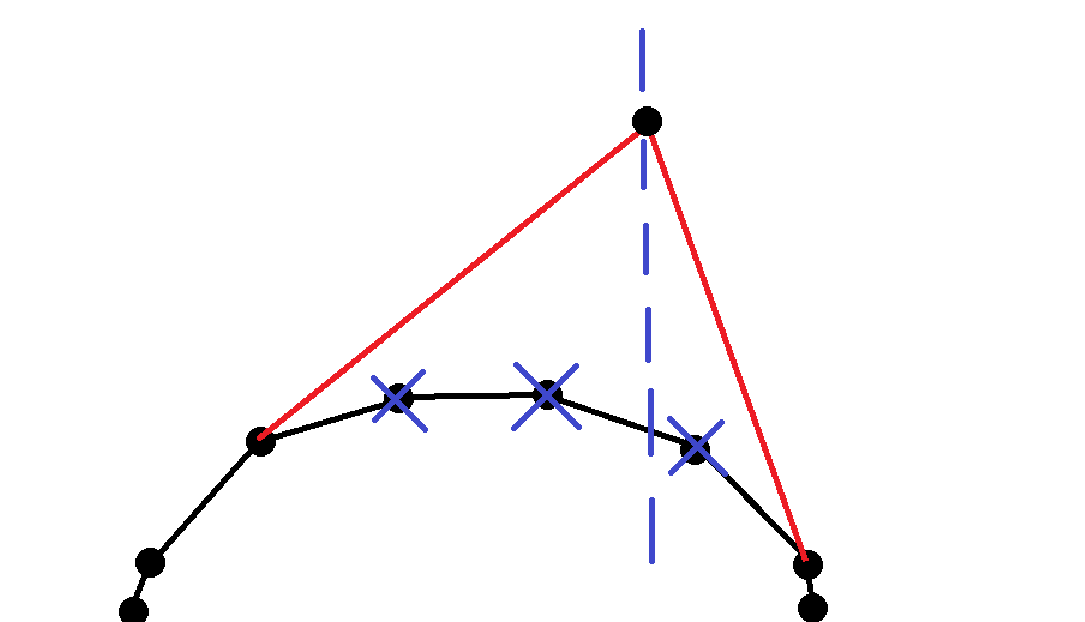
\includegraphics[width=2\linewidth]{images/49_1.png}
%\end{flushright} 
\end{minipage} \\

\textit{Асимптотически} каждое удаление и добавление по сложности занимает $O(\log n)$. Но поскольку каждая точка добавляется и удаляется не более одного раза, амортизационно будет $O(n\log n)$ в итоге. 
\newpage{}

\section{Диаметр конечного множества точек за $O(n\log n)$.}

\Task Пусть $S$ — множество точек. Нужно найти две самые далёкие точки данного множества, то есть нужно найти $\max \limits_{P, Q \in s} dist(P, Q)$.

\Statement Максимум достигается на вершинах выпуклой оболочки множества $S$. 

\Proof
Пусть максимальное расстояние достигается между точками $P$ и $Q$, причем точка $Q$ лежит внутри выпуклой оболочки. Продлим до пересечения $N$ с выпуклой оболочкой. Если это вершина, то уже все хорошо. Иначе точка попала на отрезок $AB$. Заметим, что или $AP \geq PN$, или $BP \geq PN$. 

Это можно понять из другой картинки (треугольник $XYZ$ с высотой $XH$). Там минимальное расстояние от точки $X$ до прямой достигается в $XH$, а если начать удаляться в какую-то из сторон, то расстояние будет монотонно увеличиваться. 

А т.к. хотя бы одна из точек $A, B$ более удалена от основания перпендикуляра из точки $P$ на $AB$, то в одной из них достигается расстояние не меньше, чем в $PN$, а $PN \geq PQ$.

\EndProof

\Lemma Пусть $PQ$ — диаметр $S$. Проведём прямые $l_1$ и $l_2$, перпендикулярные $PQ$, проходящие через $P$ и $Q$ соответственно. Тогда $S$ целиком лежит в полосе между $l_1$ и $l_2$.

\Proof
Пусть это не так. Тогда рассмотрим некоторую точку выпуклой оболочки, расположенную за пределами полосы между $l_1$ и $l_2$. Тогда диаметр на самом деле должен был быть больше. Противоречие. 

\EndProof

Обозначим за $l_1$ крайнюю левую вертикальную прямую, за $l_2$ — крайнюю правую вертикальную прямую. Далее начинаем синхронно вращать эти две прямые против часовой стрелки. Изменения начнутся тогда, когда одна прямая начнёт содержать одну из сторон выпуклой оболочки, тогда обновим одну из двух опорных точек. Всего таких переключений происходит $O(n)$ раз. В каждый момент переключения одной опорной точки измеряем расстояние между текущими опорными, обновляем ответ.\\

Чтобы узнать, где раньше произойдёт переключение, сравним векторные произведения. Пусть $\vec{u}$ и $\vec{v}$ — векторы, соответствующие двум сторонам. Переключение $l_1$ произойдёт раньше, если и только если $cross(\vec{u}, \vec{v}) < 0$. Это следует из свойств параллельных прямых и векторного произведения.

\Statement Пусть $ABCD$ — трапеция с основаниями $AB$ и $CD$. Тогда $\max(AC, BD) \geqslant \max(BC, AD)$.

\Proof 
Пусть не так, и без ограничения общности $BC = \max(BC, AD) > \max(AC, BD)$. Если $BC = \max(BC, AD) > AC$, то если рассмотреть перпендикуляр из точки $B$ на прямую $CD$, то $D$ лежит ближе к основанию перпендикуляра, чем $C$.  Аналогично для $BD$. Получим противоречие ($D$ лежит ближе к основанию перпендикуляра из $B$ и дальше от основания перпендикуляра из $A$, чем точка $C$). 

\EndProof

Благодаря этой лемме получим, что в случае, когда две какие-то стороны выпуклой оболочки параллельны (векторное произведение $0$, и мы не знаем, как поворачивать), поворачивать можно как угодно, т.к. мы рассмотрим обе диагонали.\\

Таким образом, в итоге будут рассмотрены все возможные кандидаты на ответ, поэтому алгоритм корректен.
\newpage{}

\section{Сумма Минковского: определение и доказательство того, что сумма Минковского двух выпуклых многоугольников — выпуклый многоугольник.}
\par \Def Пусть $M_1, M_2$ - многоугольники (со внутренностью). $M_1+M_2 = \{a+b \: | \: a \in M_1, b \in M_2\}$ - сумма Минковского
\par \Statement $M_1, M_2$ - выпуклые многоугольники $\Rightarrow M=M_1+M_2$ - выпуклый многоугольник
\par \begin{itemize}
    \item[\Proof a)] Покажем выпуклость, то есть $P,Q \in M \Rightarrow [P,Q] \in M$
    \par $P,Q \in M \Rightarrow \exists P_1, Q_1 \in M_1, P_2, Q_2 \in M_2: P_1+P_2=P, Q_1+Q_2=Q$. В силу выпуклости $M_1, M_2$ получаем, что $[P_1, Q_1] \in M_1, [P_2, Q_2] \in M_2$. Параметризуем эти отрезки:
    $$X_1 \in [P_1, Q_1] \Rightarrow X_1 = P_1 + t(Q_1-P_1), \: t \in [0;1]$$
    $$X_2 \in [P_2, Q_2] \Rightarrow X_2 = P_2 + t(Q_2 - P_2), \: t \in [0;1]$$
    \par Возьмем $X_1, X_2$ с одинаковым параметром $t$ и сложим. Таким образом можно получить любую точку отрезка $[P,Q]$. 
    $$X_1+X_2=P_1+P_2+t((Q_1+Q_2)-(P_1+P_2)) \in [P, Q] \Rightarrow [P, Q] \in M$$
    \item[b)] Покажем, что $M$ - многоугольник. Докажем, что $M_1+M_2 = conv(\{P+Q \: | P, Q$ - вершины $M_1, M_2$ соответственно$\})$
    \begin{enumerate}
        \item $M_1+M_2 \supset conv(\ldots)$ - очевидно, так как любая точка из множества в скобках лежит в $M_1+M_2$ и $M_1+M_2$ - выпуклое
        \item $M_1+M_2 \subset conv(\ldots)$. Рассмотрим точку $X+Y \in M_1+M_2, X \in M_1, Y \in M_2$
        \par Построим в кажом многоугольнике треугольник с вершинами в вершинах многоугольника, так чтобы выбранная точка лежала внутри треугольника (это возможно так как существует триангуляция). Пусть вершины треугольника для $X$ - $X_1, X_2, X_3$, для $Y$ - $Y_1, Y_2, Y_3$.
        \par \textbf{Утверждение(б/д):} $x$ лежит в $conv(\{P_1, \ldots, P_n\}) \Leftrightarrow \exists \lambda_1, \ldots, \lambda_n \geq 0: \: \sum_{i=1}^n \lambda_i = 1, \: x = \sum_{i=1}^n \lambda_i P_i$ 
        $$X=\lambda_1X_1+\lambda_2X_2+\lambda_3X_3, \: \sum_i \lambda_i=1$$
        $$Y=\mu_1Y_1+\mu_2Y_2+\mu_3Y_3, \: \sum_j \mu_j = 1$$
        $$X+Y=\sum_i \lambda_iX_i + \sum_j \mu_j Y_j=\sum_i \lambda_i(\sum_j \mu_j)X_i + \sum_j \mu_j(\sum_i \lambda_i)Y_j=\sum_{i,j} \lambda_i \mu_j (X_i+Y_j),$$$$\sum_{i,j} \lambda_i \mu_j=(\sum_i \lambda_i)(\sum_j \mu_j) = 1 \Rightarrow X+Y \in conv(\{X_i+Y_j)\})\subset conv(\ldots) \: \blacksquare$$
    \end{enumerate}
    
\end{itemize}
\newpage{}

\section{Нахождение суммы Минковского двух выпуклых многоугольников за линейное время}
\par \textbf{Алгоритм:} находим самую левую (если несколько, то выбираем самую нижнюю из них) вершину в каждом многоугольнике $M_1, M_2$ - $S_1, S_2$. Тогда $S_1+S_2$ - самая левая вершина в $M_1+M_2$. Рассматриваем векторы соответствующие ребрам $M_1,M_2$ в порядке против часовой стрелки начиная от $S_1, S_2$. Строим сумму: выбираем самое крутое из этих двух ребер (u раньше v $\Leftrightarrow$ cross(u,v)>0) и откладываем его от последней вершины суммы. Затем переходим к следующему ребру в том многоугольнике, ребро из которого мы использовали.
\par \textbf{Корректность:} Очевидно, что мы получим замкнутую ломаную (сумма всех векторов-ребер равна 0), которая является выпуклым многоугольником (из-за того что выбираем ребра именно в таком порядке по углу). Покажем, что это сумма Минковского
\par Пусть это не так: построим настоящую сумму Минковского и найдем первое ребро, которое не совпадает с нашим многоугольником. Наш многоугольник $M \subset M_1+M_2$, так как каждая вершина - сумма каких-то вершин исходных многоугольников ($S_1+S_2+[S_1, S_3]=S_3+S_2$), а значит это ребро должно лежать вне нашего многоугольника. Покажем, что такого не может быть. Пусть это ребро исходит из точки $P+Q$ и при построении нашего многоугольника было выбрано ребро $PA$ из пары $PA, QB$.
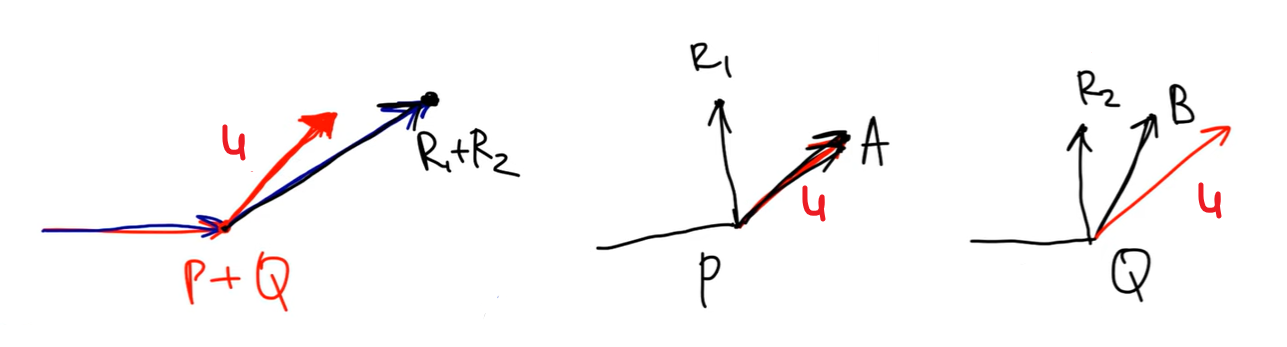
\includegraphics[width=17cm]{images/minkovsky.png}
$$PR_1+QR_2=\overline{(P+Q)(R_1+R_2)} \text{ (ребро из суммы Минковского)}$$
$$cross(PA, PR_1)\geq 0 \text{ (1)}, \: cross(QB,QR_2) \geq 0 \text{ (из рисунка)}$$
\par Так как в итоге в наш многоугольник попало ребро $PA=u$, то если отложим его от $Q$, То оно будет еще правее чем $QB$, а значит $cross(u, QR_2)\geq 0$ (2). Воспользуемся линейностью векторного произведения и сложим (1) и (2): $cross(u, PR_1+QR_2)=cross(u, \overline{(P+Q)(R_1+R_2)})\geq 0 \Rightarrow$ ребро из суммы Минковского не может лежать вне нашего многоугольника - противоречие $\Rightarrow$ построенный многоугольник совпадает с суммой Минковского
\par \textbf{Асимптотика:} $O(n+m)$, где $n,m$ - количество вершин в каждом из многоугольников.
\par \textbf{Применение*:} Поиск расстояния между выпуклыми многоугольниками: найдем $M_1-M_2=M_1+(-M_2)$ и минимальное расстояние от (0,0) до точки многоугольника. Это будет точка на какой-то стороне, поэтому просто переберм все стороны и найдем расстояние от отрезка до точки. Асимптотика: $O(n+m)$ 
\newpage{}

\section{Проверка принадлежности точки многоугольнику: решение с помощью суммы ориентированных углов.}
\par \textbf{Алгоритм:} находим сумму ориентированных углов $APB$, где $P$ - рассматриваемая точка, $AB$ - ребро нашего многоугольника в порядке какого-то обхода. \begin{enumerate}
    \item Сумма равна 0: точка снаружи
    \par 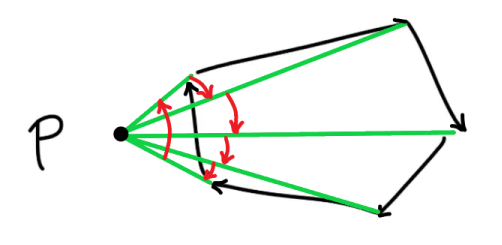
\includegraphics[width=10cm]{images/point_in_polygon_sum_0.png}
    \item Сумма равна $\pm 2\pi$: точка внутри
    \par 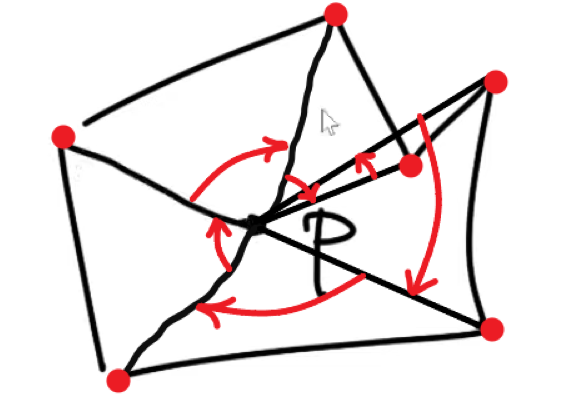
\includegraphics[width=10cm]{images/point_in_polygon_sum_2pi.png}
\end{enumerate}
\par \textbf{Проблемы:} используем тригонометрию (долго работает), работаем с double (если точек много, то можем настолько потерять точность, что не отличим 0 от $2\pi$)
\newpage{}

\section{Проверка принадлежности точки многоугольнику: решение с горизонтальным лучом. Модификации: случайный луч, луч, заведомо не содержащий вершин многоугольника.}

Рассмотрим оптимизацию предыдущего алгоритма. 
Посмотрим на точку в многоугольнике и выпустим из неё горизонтальный луч вправо. Идея простая: если число пересечений луча с границами многоугольника чётное, то точка лежит вне многоугольника, а если нечётное, то внутри. 

\par \textbf{Проблема:} вершины многоугольника могут попасть на луч, и тогда результат не определён.

\par \textbf{Решение 1:} вместо горизонтального луча мы пускаем случайный луч.
\par \textbf{Проблема:} рандомизированный алгоритм и использование double.

\par \textbf{Решение 2:} Пусть все точки имеют целочисленные координаты, где $0 \leq x, y \leq A$. Давайте пустим из точки p вектор с координатами $(A, A+1)$, тогда на таком векторе нет ни одной вершины многоугольника.

Доказательство: пусть такая точка лежит на отрезке но координаты нашего вектора это взаимно простые числа, и если у какой-то из вершин многоугольника координаты $(x_0, y_0)$ всё-таки лежат на векторе, то 
\[(x - p.x,\; y- p.y) \;|| \;(A, \;A+1)\]
Значит, они отличаются на константу $\lambda \geq 0$. Но если $\lambda$ целое, то мы выходим за ограничение $0 \leq x, y \leq A$.
\par \textbf{Проблема:} Необходимо знать верхнеее ограничение на $A$.

\par \textbf{Решение 3:} Пускать горизонтальный луч и обрабатывать вершины прямоугольника.

Пусть $(a, b)$ это сторона многоугольника. При необходимости переставим концы местами так чтобы выполнялось неравенств $b.y \geq a.y$.

Если $(b.y \leq p.y || a.y > p.y)$, то continue. То есть сторона целиком лежит над лучом. А первый случай - либо отрезок целиком строго снизу, либо, возможно, он просто касается, или же целиком лежит на стороне. В этих случаях мы игнорируем.


\begin{lstlisting}
  if (b.y <= p.y || a.y > p.y) {
    continue;
  }
  if (cross(p - a, b - a) < 0) {
    ++cnt;
  }
\end{lstlisting}

Здесь $cnt$ — количество пересечений. Работоспособность показывается через перебор случаев.

\begin{lstlisting}
  if (cnt % 2 == 1) {
    cout << "p is in our figure" << endl;
  } else {
    cout << "p is not in our figure" << endl;
  }
\end{lstlisting}

\Note Нужно отдельно проверить, не лежит ли точка $p$ на границе многоугольника.
\newpage{}

\section{Пересечение полуплоскостей: алгоритм за $O(n^2)$}
Постановка задачи: дано $n$ полуплоскостей, необходимо найти их пересечение.

В большинстве случаев получается выпуклый многоугольник. Выпуклость следует из того, что эта фигура — пересечение выпуклых фигур. Однако может получиться и неограниченная выпуклая фигура.

Представление полуплоскостей: 
Прямую храним в виде чисел $a$, $b$, $c$ таких, что $ax + by + c = 0$. Полуплоскость можно хранить в виде таких же чисел, что $ax + by + c \geqslant 0$. Альтернативно можно хранить нормаль к прямой. Векторы нормалей нормированы, то есть $a^2 + b^2 = 1$.

\Note Считаем, что в множестве полуплоскостей $x$, $y$ не превосходят некоторого числа $inf = 10^9$ по модулю. Этот приём называется bounding box, и широкое применение он получил в разработке компьютерных игр.

Изначально посмотрим на bounding box, затем пройдём по всем полуплоскостям в произвольном порядке, и «отрезаем» часть, которую не принадлежит полуплоскости. Храним выпуклый многоугольник, который является временным ответом, и для любого $i$ пересекаем этот многоугольник с $i$-й полуплоскостью. В многоугольнике $O(n)$ вершин, пересечение полуплоскостью происходит за $O(n)$, и итоговая асимптотика выходит $O(n^2)$.

Если для любой вершины $v$ многоугольника $a \cdot v.x + b \cdot v.y + c \geqslant 0$, то менять ничего не нужно. Если же для любой вершины $v$ выполняется, что $a \cdot v.x + b \cdot v.y + c < 0$, то ответом будет пустое множество

\section{Пересечение полуплоскостей: алгоритм за $O(n log n)$.}
Давайте все полуплоскости разобьём на два класса: 
У первого типа полуплоскостей нормаль лежит под углом $[0, \pi)$, у второго класса $[\pi, 2\pi)$. 


Если пересечь все полуплоскости первого класса, то получится в некотором смысле нижняя огибающая нашего ответа. Если аналогично пересечь все полуплоскости второго класса, то получится верхняя огибающая нашего ответа.

Внутри каждого класса отсортируем все полуплоскости по углу нормали, используя векторное произведение. Сортировка происходит за $O (n \log n)$. Далее объединим отсортированные списки полуплоскостей в один.

\Note Если сортировать исходный список, то предикат с векторным произведением не сработал бы.

Отсортированный список полуплоскостей храним в деке (deque, double ended queue). В цикле по $i$ от $0$ до $n - 1$ делаем следующее: пока в деке есть хотя бы две полуплоскости и точка пересечения двух последних не лежит в $h_i$, то делаем $deque.pop\_back();$, далее аналогично делаем $deque.pop\_front();$, затем делаем $deque.push\_back(h_i)$. После делаем ещё два цикла $while$, но на этот раз пока в деке хотя бы три полуплоскости, и точка пересечения последних двух не лежит в первой, то извлекаем с конца, пока в деке хотя бы три полуплоскости, и точка пересечения первых двух не лежит в последней, то извлекаем с начала. Если в деке осталось не более двух полуплоскостей, то ответ пуст. Иначе в деке лежат стороны искомого многоугольника.

Что делать с прямыми, у которых нормали параллельны? Среди полуплоскостей с одним и тем же вектором нормали оставляем только полуплоскость с наименьшим $c$.

\newpage{}

\section{Post office problem: постановка. Определение диаграммы Вороного. Алгоритм построения за $O(n^2log n)$. Вид каждой ячейки диаграммы.}
\textbf{Постановка проблемы}: Давайте представим, что мы живем в какой-то стране, страна расположена на плоскости, нет никаких препятсвий в виде столбов и зданий... то есть расстояние между двумя точками - это просто евклидово расстояние между точками. У нас есть n почтовых отделений. И нужно понять: если человек хочет отправить какое-то письмо, в какое самое близкое почтовое отделение ему нужно пройти?
\\
\\
Понятно, что наша плоскость разобьется на n регионов, и в каждой области будет лишь одно самое близкое почтовое отделение
\\
\\
\textbf{Определение} Точки в нашем городе по умолчанию называюсся \textit{сайтами}
\\
\\
\textbf{Определение} \textit{Диаграмма Вороного} конечного множества точек S на плоскости представляет такое разбиение плоскости, при котором каждая область этого разбиения образует множество точек, более близких к одному из элементов множества S, чем к любому другому элементу множества
\\
Наивный алгоритм построения:
\begin{itemize}
    \item Для каждой точки i выполним следующее:
    \begin{itemize}
        \item Проведем n-1 плоскость, j-ая из которых будет определяться как серединный перпендикуляр к отрезку [i, j], $i \neq j$, причем нормаль этой плоскости ориентирована к точке i
        \item Пересечем все эти плоскости, используя алгоритм за O(n log n) и получим ячейку диаграммы Вороного
    \end{itemize}
\end{itemize}
\textit{Асимптотика $O(n^2 logn)$}
\\
\textbf{Следствие} \\ Каждая ячейка диаграммы Вороного - выпуклая фигура, т.к. пересечение полуплоскостей - выпуклая фигура, обобщенный выпуклый многоугольник (то есть он может быть неограниченным с какой-то стороны)
\newpage{}

\section{Связность диаграммы Вороного. Число вершин и рёбер в диаграмме.}
\textbf{Утверждение}
\begin{itemize}
    \item Если все сайти лежат на одной прямой, то диаграмма Вороного $Vor(P)$ состоит из (n-1) параллельной прямой
     \item В противнойм слуае ребрами $Vor(P)$ могут выступать только отрезки или лучи, причем $Vor(P)$ связна, если ее воспринимать, как граф
\end{itemize}
$\blacktriangle$ \\ 
1. Исходя из алгоритма построения диаграммы Вороного за $O(n^2 logn)$ получим, что если точки располагаются на одной прямой, то границы ячеек диаграммы - это просто серединные перпендикуляры к отрезкам между ближайшими точками\\
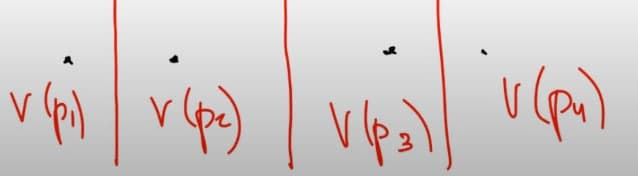
\includegraphics[width=10cm]{polina3.jpg}
\\
\\
2. Пусть не все точки лежат на одной прямой. Покажем, что в таком случае не бывает прямых, а бывают только отрезки и лучи.
\\
Предположим, это не так, и прямая возникла. Тогда картинка какая-то такая. Пусть есть две точки $p_i, p_j$, между которыми проведен серединный перпендикуляр, являющийся, собственно, прямой-границей диаграммы Вороного. 
\\
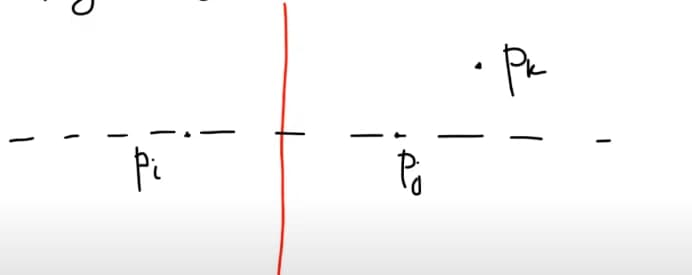
\includegraphics[width=10cm]{polina4.jpg}
\\
Мы знаем, чт не все точки лежат на одной прямой. Это значит, что вне прямой $p_ip_j$ есть хотябы одна точка. БОО пусть она лежит тут(точка $p_k$). Серединный перпендикуляр между точками  $p_jp_k$ не параллелен серединному перпендикуляру между точками $p_ip_j$, значит, эти перпендикуляры пересекутся.
\\
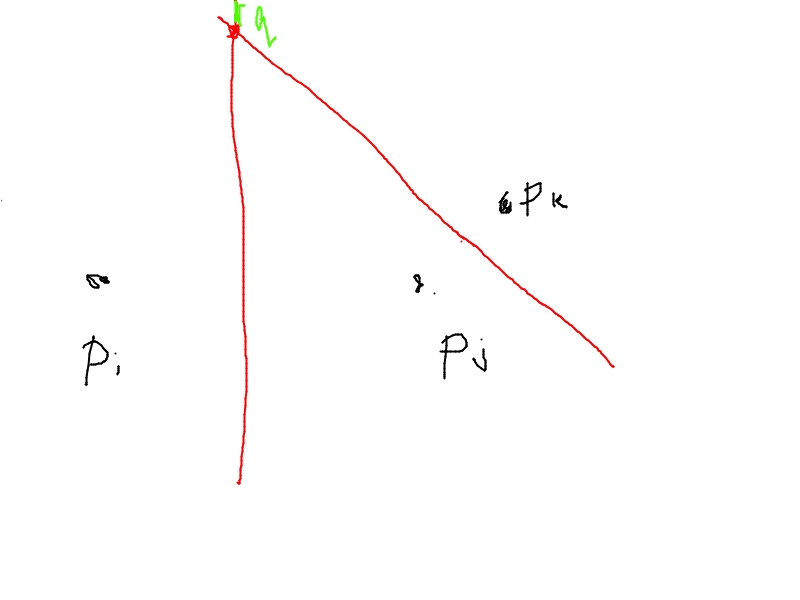
\includegraphics[width=10cm]{polina5.jpg}
\\
Отсюда мы делаем вывод, что точки из q ближе к $p_k$ чем к $p_j$. Но тогда прямая не может лежать целиком в диаграмме Вороного. Противоречие.
\\
\\
Отсюда следует, что ребрами в диаграмме Вороного могут выступать только отрезки и лучи.
\\
\\
Отсюда так же следует, что диаграмма Вороного связна. Предположим, что это не так. Тогда единственный случай, когда это может выполняться - если в диаграмме Вороного какая-то из ячеек ограничена с двух сторон параллельными прямыми, что противоречит только что доказанному утверждению.\\$\blacksquare$

Из этого утверждения следует Теорема:
\\
\textbf{Теорема}\\
Если $n \geq 3$ и не все сайты лежат на одной прямой, то $Vor(P)$ содержит не более $2n - 5$ вершин и $3n - 6$ ребер
\\
$\blacktriangle \\$ Возьмем какую-нибудь фиктивную вершинку $V_{\infty}$, на которую замкнем без пересечений некоторые ребра так, чтобы у нас не возникало бесконечных областей диаграммы, сформированных бесконечными лучами. Теперь у нас получился конечный граф, для которого применима формула Эйлера. По предыдущему утверждению граф связен, поэтому формула Эйлера применима \\
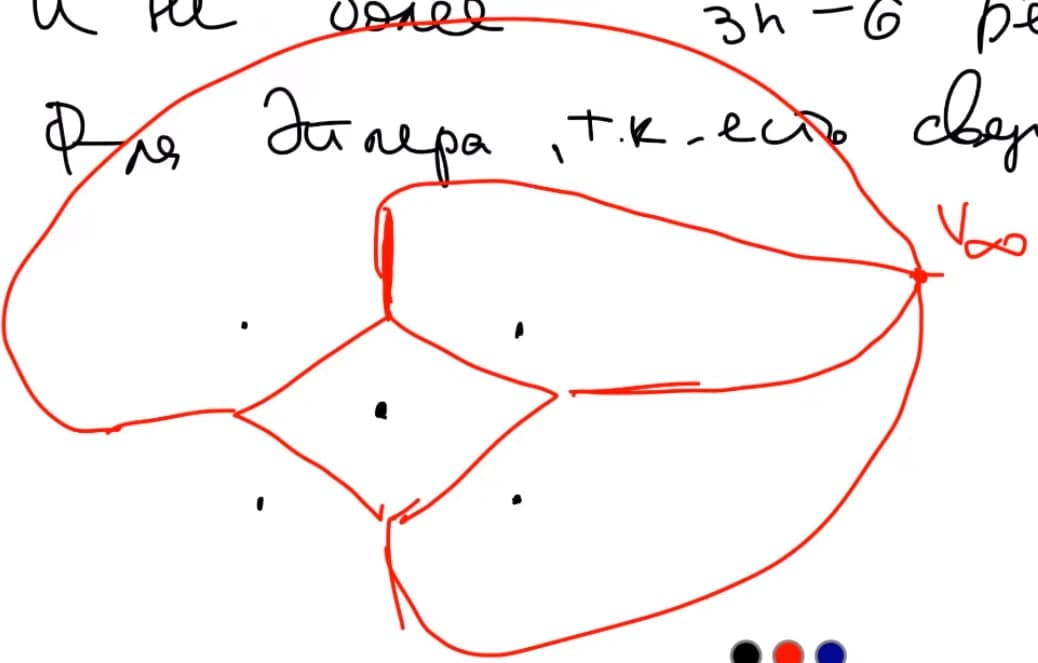
\includegraphics[width=10cm]{polina6.jpg} \\
$v+1$ - вершин \\
$e$ - ребер \\
$n$ -граней
\\
\\
$v+1+n-e = 2$
\\
$v+n-e = 1$
\\
Воспользуемся оценкой, что $2e \geq 3(v+1)$ ($2e$ - сумма степеней всех вершин по леммме о рукопожатиях, при этом у каждой вершины степень как минимум 3.
\\
Для обычных вершин это очевидно. Так как если у какой-то вершинки было бы всего два ребра, то один из углов, образованных этими углами, был бы >= 180, чего не может быть,так как каждая ячейка диаграммы Вороного - выпуклая фигура
\\
Примерно то же самое для вершины $V_{\infty}$. Все лучи заметают угол $2\pi$, и в силу этого их должно быть хотябы три)
\\
\\
$v = e + 1 - n, v \leq \frac{2e -3}{3} \Longrightarrow e + 1 - n \leq \frac{2e -3}{3} \Longrightarrow \frac{e}{3} +2 - n \leq 0 \Longrightarrow e \leq 3n - 6$
\\
$e \geq  \frac{3v+3}{2}, e = v+n-1 \Longrightarrow v + n - 1 \geq \frac{3v+3}{2}  \Longrightarrow \frac{v}{2} + \frac{5}{2} \leq n \Longrightarrow v \leq 2n-5$
\\
$\blacksquare$
\newpage{}

\section{Критерий того, что точка является вершиной диаграммы Вороного. Критерий того, что серединный перпендикуляр к $p_ip_j$ участвует в диаграмме Вороного.}
\textbf{Определение} Пусть $P$ — набор сайтов, точка $q$ лежит на плоскости. Тогда $C_q(P)$ — круг максимального радиуса с центром в точке $q$, который во внутренности не содержит ни одного сайта.
\\
\\
\textbf{Теорема} \\
\begin{itemize}
    \item Точка $q$ является вершиной диаграммы Вороного $Vor(P)$ тогда и только тогда, когда $C_q (P)$ содержит на своей границе хотя бы три сайта
    \item В диаграмме Вороного $Vor (P)$ участвует серединный перпендикуляр к отрезку $p_i p_j$ тогда и только тогда, когда существует точка $q$, лежащая на серединном перпендикуляре к отрезку $p_i p_j$,  такая что $C_q (P)$ содержит на границе $p_i$ и $p_j$, и больше никакие точки не содержит ни внутри, ни на границе.
\end{itemize}
$\blacktriangle$\\
1.

$\Longrightarrow$ Для любой вершины $q$ диаграммы Вороного выполнено, что её степень хотя бы $3$, значит, $q$ лежит на границе хотя бы трёх ячеек диаграммы Вороного. 
\\
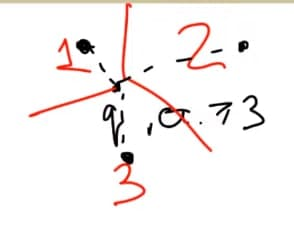
\includegraphics[width=6cm]{polina7.jpg}
\\
Значит, точка $q$ равноудалена от хотя бы трёх сайтов, которые порождают эти ячейки. Если есть более близкий сайт, точка $q$ не могла лежать в трёх исходных ячейках. Хотябы потому, что тогда одна из точек образовывала бы другую ячейку, в которой точка $q$ не лежит.

$\Longleftarrow$ Рассмотрим точку $q$ и такой круг $C_q (P)$, что на его границе хотя бы три сайта. Тогда точка $q$ лежит на пересечении серединных перпендикуляров, и к $q$ есть хотя бы три самых близких сайта, но тогда $q$ лежит хотя бы на трёх ячейках, и $q$ — вершина всех этих ячеек по построению. \\
2.
\\
$\Longrightarrow$ Рассмотрим серединный перпендикуляр к отрезку $p_i p_j$, выберем в качестве точки $q$ любую внутреннюю точку той части перпендикуляра, которая участвует в диаграмме Вороного. Рассмотрим круг с центром в точке $q$ и радиусом $q p_j$. Круг также содержит $p_i$. Круг пуст, иначе к $q$ есть более близкий сайт. На границе круга больше нет других сайтов, так как иначе $q$ по первому утверждению должна быть вершиной диаграммы Вороного $Vor (P)$.

$\Longleftarrow$ Пусть существует точка $q$, лежащая на серединном перпендикуляре к отрезку $p_i p_j$,  такая что $C_q (P)$ содержит на границе $p_i$ и $p_j$, и больше никакие точки не содержит ни внутри, ни на границе. Тогда самые близкие точки к $q$ — это точки $p_i$ и $p_j$, остальные находятся строго дальше. Тогда окрестность точки $q$ является общей частью границы ячеек $V (p_i)$ и $V (p_j)$.
\\
$\blacksquare$
\newpage{}

\section{Описание алгоритма Форчуна, два типа событий. Асимптотика.}
Алгоритм основан на принципе сканирующей прямой. Сканирующая прямая будет идти сверху вниз. Идея таковая: пусть $l$ — текущая прямая, рассмотрим сайты выше неё и ниже неё, тогда диаграмма Вороного корректно построена для множества таких точек, что расстояние от них до какого-либо из сайтов меньше, чем расстояние до прямой.
\\
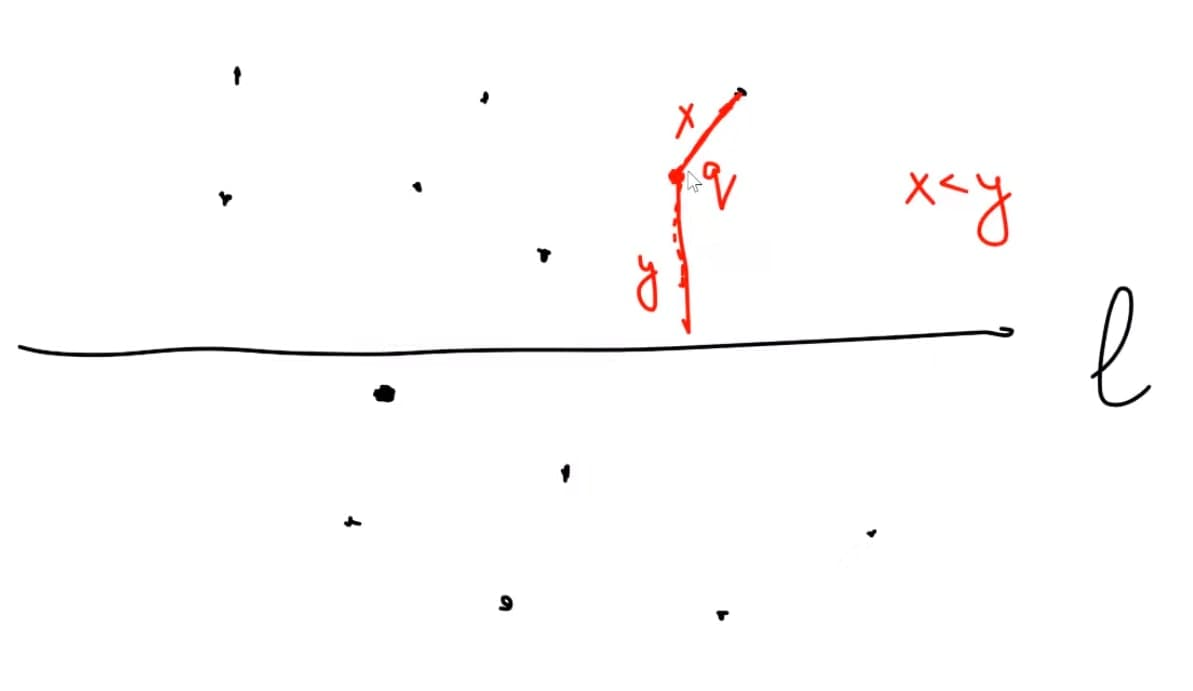
\includegraphics[width=10cm]{polina8.jpg}
\\
Множество точек, равноудаленных он данной прямой и данной точки - парабола. Тогда сайт $p_i$ будет фокусом параболы, а $l$ — её директрисой, и внутренняя часть параболы - это та часть плоскости, для которой мы точно знаем ответ.
\\
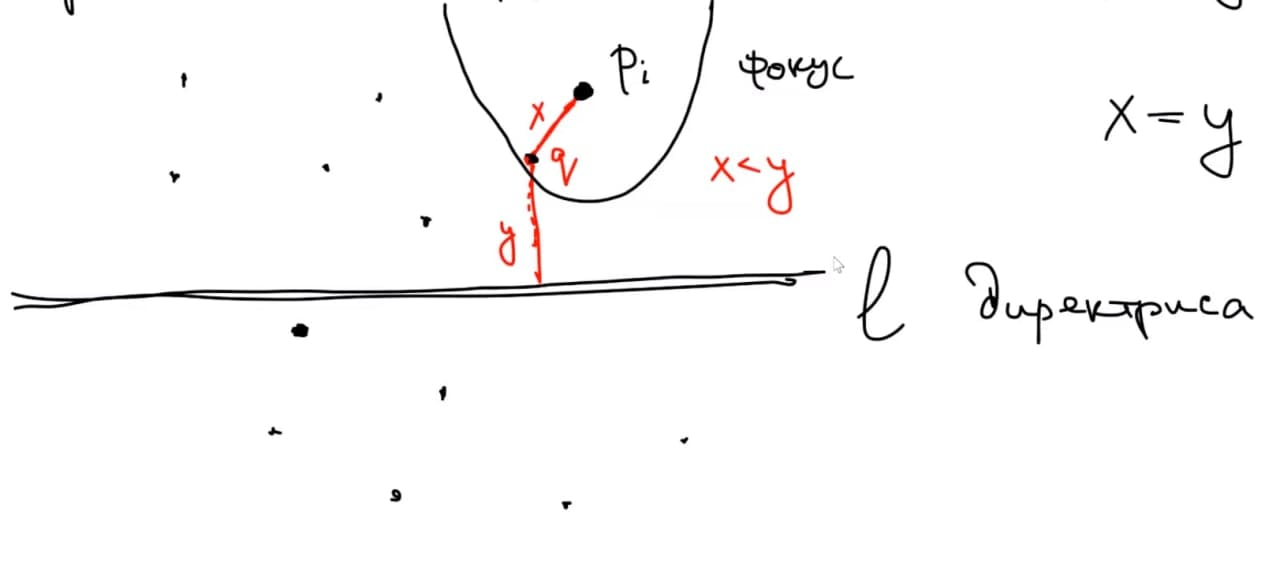
\includegraphics[width=10cm]{polina9.jpg}
\\
Построим для каждого сайта такую параболу и рассмотрим их нижнюю огибающую. Все эти параболы в совокупности образуют береговую линию (beach line). 
\\
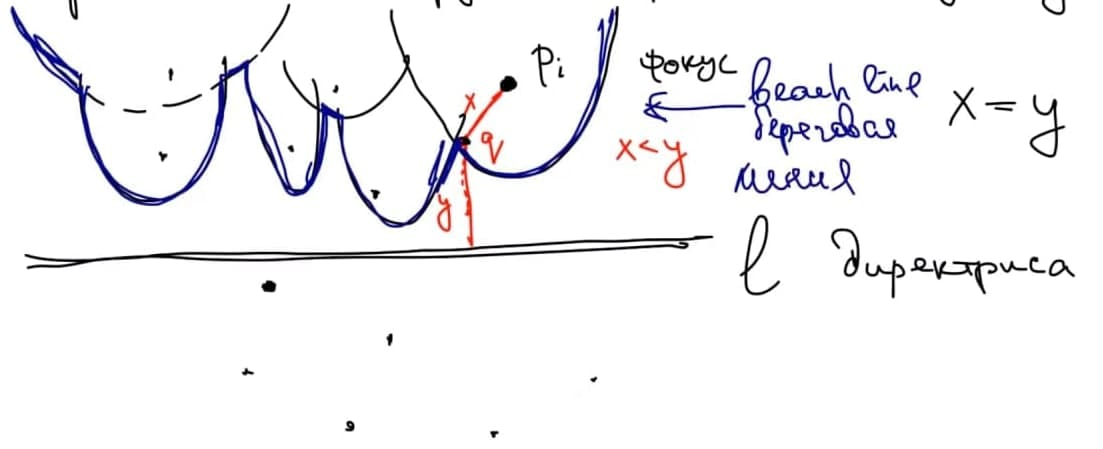
\includegraphics[width=10cm]{polina10.jpg}
\\
Как меняется эта береговая линия по мере спуска прямой? Рассмотрим два события
\begin{itemize}
    \item [1] Рассмотрим момент, когда обрабатывается новый сайт (site event, событие-точка). Появляется новая парабола, изначально вырождающаяся в луч, и она вставляется в береговую линию.
     \item [2] Второй тип события - circle event, возникающий, когда параболу надо удалить из береговой линии. Это происходит тогда, когда одна из парабол вырождается в точку
     \\
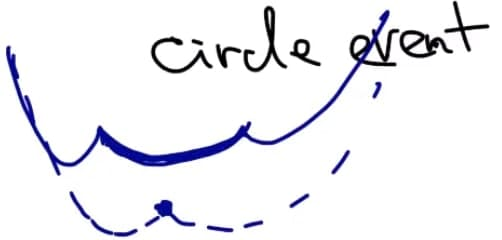
\includegraphics[width=6cm]{polina11.jpg}
\\
Почему это circle event? Потому что на самом деле эта точка будет вершиной диаграммы Вороного, ведь она равноудалена от фокуса как минимум трех парабол и директриссы. Для этого случая мы смотрим на все тройки подряд идущих дуг парабол, вычисляем точку, равноудалённую от трёх фокусов (строим центр описанной окружности соответствующего треугольника) и говорим, что если эта точка находитя на расстоянии $r$(радиус полученной окружности) от прямой, то нужно добавить новое событие, при котором появляется вершина диаграммы Вороного и одна из дуг удаляется.

\end{itemize}
Пересечения парабол из береговой линии на самом деле вычерчивают ребра диаграммы Вороного. В какой-то момент ребра пересекаются, какая-то из дуг схлопывается, и мы получаем вершинку.
\\
\\
Соответственно, наш алгоритм просто идет аккуратно сверху вниз, поддерживает все события, которые будут происходить. Для всех трех подряд идущих параболок поддерживает точку пересечения. Заводит себе событие, что если прямая $l$ дошла до уровня, что расстояние до нее от центра окружности совпадает с радиусом соответствующей описанной окружности, то появляется circle event, и необходимо как-то аккуратно удалить параболу, провести новые ребра диаграммы Вороного.
\\
 Ну а если сайтовая ситуация, то нужно добавить новую параболу (изначально луч), понять, где она пересекает береговую линию, изменить береговую линию с учетом этой новой параболы.
 \\
 \\
 Потом перебрать снова тройки параболы. Обработать circle event, если он возник, и если это так, добавить его в очередь событий
\\
\\
Всего $O(n)$ событий, так как каждое событие - это либо вершина диаграммы Вороного, либо один из сайтов.
\\
Обработка событий идёт с помощью дерева поиска на статусе, и все события вставки/удаления, порожденные circle event и site event, можо делать с помощью него за $O(log n)$
\\
\\
Таким образом, асимптотика алгоритма $O(n log n)$

\newpage{}

\section{Определение триангуляции. Мотивировка: моделирование ландшафта. Число треугольников и рёбер в триангуляции.}

Пусть $P = \{p_1, \dots, p_n \}$ - набор сайтов; 

\Def Триангуляция -- набор попарно пересеющихся по внутренности треугольников с вершинами в сайтах, объединение которых равно выпуклой оболочке множества сайтов ($Conv(P)$).


\textbf{Мотивировка:} есть карта местности, где для точек известна высота. По этим измерениям хочется представить настоящий ландшафт.

\textbf{Cпособ 1}: построить диаграмму Вороного, многоугольники поднять на высоту соответствующей точки. \textit{Минус:} дискретность и разрывы. 

\textbf{Способ 2}: триангуляция, и вот эти треугольники как-то ставить линейной функцией в пространстве; 

проблема: слишком тонкие треугольники - если у треугольника маленькие углы, он с большей вероятностью соединяет далёкие точки разной высоты, следовательно, представляться ландшафт будет хуже. Будем максимизировать эту величину. (Задача: найти триангуляцию, где минимальный угол максимален).

Пусть есть триангуляция множества из n сайтов, на границе $conv(P)$ k сайтов, не все сайты на одной прямой $\Rightarrow$ тогда в трианг. \textbf{2n - 2 - k треугольников и 3n - 3 - k рёбер}.

$\blacktriangle$ Формула Эйлера: граф связный (очевидно), n вершин, m треугольников (треугольники == грани + ещё одна грань - бесконечная) -> $n - Edges + m + 1 = 2$; но мы знаем, что $Edges = \frac{3m+k}{2}$ (очевидно), решаем линейное уравнение. $\blacksquare$.

\section{Определение графа Делоне, его свойство. Критерий того, что три сайта являются вершинами одной грани графа Делоне (б/д). Критерий того, что два сайта соединены ребром в графе Делоне (б/д). Определение триангуляции Делоне.}

Пусть P - набор сайтов, Vor(P) - диаграмма Вороного.


\Def Граф Делоне  — граф, где вершины - сайты,а рёбра соединяют сайты, ячейки которых имеют общую сторону в виде ребра или луча. \\

\textbf{Утверждение:} Граф Делоне - плоский (планарный) укладка графа называется плоской, если рёбра пересекаются только по вершинам.
Граф называется планарным, если у него существует плоская укладка.

$\blacktriangle$ Пусть не так, пусть $p_i p_j$ и $p_k p_l$ — пересекающиеся рёбра графа Делоне. Так как $p_i p_j$ — ребро, то существует круг с центром в точке $x_{ij}$, такой что на границе лежат $p_i$, $p_j$ и только они, и внутри нет точек. Интервал $x_{ij} p_i$ является подмножеством $V (p_i)$. Ни одна вершина треугольника $T_{kl}$ не лежит внутри $T_{ij}$. Аналогично ни одна вершина треугольника $T_{ij}$ не лежит внутри $T_{kl}$. Тогда один из отрезков $p_i x_{ij}$ и $p_j x_{ij}$ пересекает один из отрезков $p_k x_{kl}$ и $p_l x_{kl}$. Но это означает, что две ячейки диаграммы Вороного пересекаются по внутренности. Противоречие. $\blacksquare$

\begin{enumerate}
    \item Сайты $p_i$, $p_j$, $p_k$ - вершины одной (ограниченной) грани графа Делоне $\Leftrightarrow$ $\exists$ точка $q$, такая что $C_q (P)$ содержит на границе точки $p_i$, $p_j$, $p_k$;
    \item Отрезок $p_i p_j$ - ребро графа Делоне $\Leftrightarrow$ $\exists$ точка $q$ на серединном перпендикуляре к отрезку $p_i p_j$, такая что $C_q (P)$ содержит на границе точки $p_i$ и $p_j$ и больше никого.
\end{enumerate}

\textbf{Триангуляция Делоне} — любая триангуляция, полученная из графа Делоне подразбиением всех граней на треугольники.
\newpage{}

\section{Флип ребра. Нелегальное ребро, критерий легальности (б/д). Проверка легальности в терминах определителя (б/д).}

Пусть в триангуляции $T$ есть два треугольника $\triangle p_i p_j p_k$ и $\triangle p_i p_j p_l$, и их объединение — выпуклый четырёхугольник. Тогда операция $edge \ flip$ преобразует разбиение выпуклого четырёхугольника из двух треугольников $\triangle p_i p_j p_k$ и $\triangle p_i p_j p_l$ в $\triangle p_i p_k p_l$ и $\triangle p_j p_k p_l$.

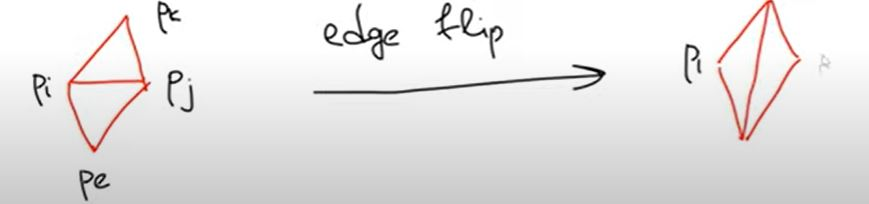
\includegraphics[width=10cm]{images/flip.JPG}

Ребро $p_i p_j$ называется \textbf{нелегальным}, если после операции $edge \ flip$ над ребром $p_i p_j$ минимальный угол увеличился (как на картинке).

\textbf{Критерий нелегальности}: Пусть в триангуляции $T$ есть два треугольника $\triangle p_i p_j p_k$ и $\triangle p_i p_j p_l$. Тогда ребро $p_i p_j$ нелегально тогда и только тогда, когда круг, описанный вокруг $p_i p_j p_k$ содержит $p_l$ строго внутри.

\textbf{Проверка легальности}:

Пусть $p$, $q$, $r$ — вершины треугольника, заданные при обходе по часовой стрелке. Тогда точка $s$ лежит внутри круга, описанного вокруг треугольника, тогда и только тогда, когда следующий определитель положителен:

\begin{center}
    $\begin{vmatrix} p_x & p_y & p_x^2 + p_y^2 & 1 \\ q_x & q_y & q_x^2 + q_y^2 & 1 \\ r_x & r_y & r_x^2 + r_y^2 & 1 \\ s_x & s_y & s_x^2 + s_y^2 & 1 \end{vmatrix}$
\end{center}

\section{Легальная триангуляция, легализация триангуляции. Критерии триангуляции Делоне (б/д). Максимизация минимального угла в триангуляции Делоне.}
\textbf{Легальная триангуляция} - та, в которой нет нелегальных рёбер.

\textbf{Критерии триангуляции Делоне}:
\begin{enumerate}
    \item Триангуляция $T$ - т. Делоне $\Leftrightarrow$ круг, описанный вокруг любого треугольника из $T$ не содержит внутри себя других вершин триангуляции.
    \item  Триангуляция $T$ - т. Делоне $\Leftrightarrow$ $T$ триангуляция легальна.
\end{enumerate}

Триангуляция Делоне максимизирует минимальный угол.

$\blacktriangle$ Пусть $T$ — триангуляция Делоне с минимальным углом $\alpha$, $T'$ — другая триангуляция с минимальным углом $\beta > \alpha$. Легализуем $T'$, получим $T''$ с минимальным углом $\gamma \geqslant \beta > \alpha$. $T''$ — тоже триангуляция Делоне. Но минимальные углы триангуляций Делоне получились разными, а должны быть одинаковыми. Противоречие. $\blacksquare$

\newpage{}

\section{Рандомизированный алгоритм построения триангуляции Делоне: описание, асимптотика (б/д).}

Алгоритм будет итеративным рандомизированным (вероятностным). Возьмём самую высокую точку $p_0$ в множестве сайтов $P$, среди нескольких точек с наибольшим $y$ возьмём точку с наибольшим $x$. Возьмём фиктивныые точки $p_{-1}$ и $p_{-2}$ так, чтобы внутри треугольника $\triangle p_0 p_{-1} p_{-2}$ оказались все оставшиеся сайты. Далее перемешаем сайты в случайном порядке. Поддержим легальную триангуляцию для множества сайтов $\{ p_{-2}, p_{-1}, \dots, p_{r - 1} \}$ Если точка попала в треугольник, то разобьём этот треугольник на ещё несколько треугольников. Если ранее легальное ребро оказалось нелегальным, то это связано только с этой попавшей точкой. Выполним операцию $edge \ flip$. Проверим далее легальность других рёбер, и так до тех пор, пока не восстановится легальность.

Этот алгоритм конечный. Легализаций происходит $n$ раз.

\textbf{Асимптотика}: Математическое ожидание времени работы алгоритма есть $O (n \log n)$, при этом количество операций $edge \ flip$ в среднем $O (n)$, причём основная сложность - это локализация точки.

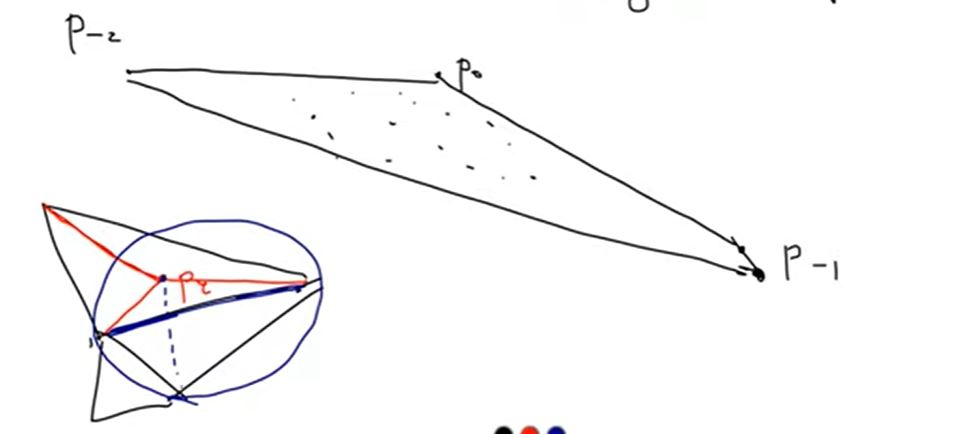
\includegraphics[width=10cm]{delone.JPG}

\begin{lstlisting}
random_shuffle(p[1], p[2], ..., p[n - 1]);
for r = 1, ..., n - 1:
  if (IsInside(p[r], Triangle(p[i], p[j], p[k]))) {
    DeleteTriangle(p[i], p[j], p[k]);
    AddTriangle(p[i], p[r], p[k]);
    AddTriangle(p[i], p[j], p[r]);
    AddTriangle(p[j], p[k], p[r]);
    LegalizeEdge(p[r], p[i], p[j]);
    LegalizeEdge(p[r], p[j], p[k]);
    LegalizeEdge(p[r], p[k], p[i]);
  }
  if (IsBorderPoint(p[r], Triangle(p[i], p[j], p[k]), Triangle(p[j], p[i], p[l]))) {
    delete 2 old triangles;
    add 4 new triangles;
    legalize 4 edges;
  }
\end{lstlisting}

После завершения всех легализаций рёбер получим легальную триангуляцию.

$\blacktriangle$ Это следует из того, что добавляемые рёбра одной из вершин содержат $p_r$. Такие рёбра обязательно лежат в графе Делоне. Остаётся доказать, почему утверждение о рёбрах выполняется. $\blacksquare$
\newpage{}

\section{Триангуляция Делоне: процедура legalizeEdge, реализация.}
\begin{lstlisting}
LegalizeEdge(Point pr, Point pi, Point pj):
  Point pk; // vertex of the second triangle;
  if (IsIllegal(pi, pj)) {
    delete 2 old triangles;
    add 2 new triangles;
    LegalizeEdge(pr, pi, pk);
    LegalizeEdge(pr, pk, pj);
  }
\end{lstlisting}

\section{Триангуляция Делоне: решение задачи локализации.}

\textbf{В каком треугольнике(-ах) лежит $p_r$?}

Решение: Храним историю триангуляции в виде ориентированного ациклического графа. Каждая вершина такого графа соответствует треугольнику, который когда-то существовал. Треугольник может разбиться на три треугольника. После переворачивания ребра из вершин, соответствующих двум старым треугольникам, проведём рёбра в одни и те же две вершины, соответствующим новым треугольникам.

Процесс локализации происходит в несколько шагов:

1) Встать в корень;

2) Спуститься в такой дочерний треугольник, где лежит $p_r$;

3) Завершиться в листе, соответствующем треугольнику текущей триангуляции.

За счёт случайного порядка $p_1$, $\dots$, $p_{n - 1}$ граф будет иметь в среднем логарифмическую глубину.

\section{Триангуляция Делоне: обработка точек p-2, p-1 (б/д).}

Будем говорить, что точка $p$ находится выше точки $q$, если либо $p.y > q.y$, либо при $p.y = q.y$ $p.x < q.x$.

Формально, $p_{-1}$ — точка ниже всех точек $P$, такая что из неё все точки в порядке обхода по часовой стрелке видны в порядке высоты. $p_{-1}$ расположен настолько далеко, что не лежит ни в одном круге, построенным по трём точкам из $P$. 

Формально говоря, $p_{-2}$ — точка выше всех точек $P$, что из неё в порядке обхода против часовой стрелки все точки из $P \cup \{  p_{-1} \}$ видны в порядке возрастания высоты. $p_{-2}$ расположена достаточно далеко, что $p_{-2}$ находится вне любого круга, построенного по трём точкам из $P \cup p_{-1}$.

Далее проверим легальность.

Возможно несколько случаев:

1) Если $p_i p_j$ — ребро треугольника $p_{-2} p_0 p_{-1}$, то $p_i p_j$ легально;

2) Если $i$, $j$, $k$, $l \geqslant 0$, то делаем обычную проверку через определитель;

3) $p_i p_j$ легально тогда и только тогда, когда $\min(k, l) < \min (i, j)$, среди $i$, $j$ — не больше одного отрицательного, $k$, $l$ — хотя бы одна — $p_r$ — не больше одного отрицательного.